%!TEX root = ../../dissertation.tex
%%%%%%%%%%%%%%%%%%%%%%%%%%%%%%%%%%%%%%%%%%%%%%%%%%%%%%%%%%%%%%%%%%%%%%%%%%%%%%%%
\chapter{Video Streaming Techniques}
\label{chap:streaming}

\begin{itemize}
\item Introduction. Streaming, Popularity. Chapter Intention.
\item Technical Background. Reliable and Unreliable Streaming. Realtime and Stored Streaming.
\item Protocol Overview. Transport and Application Layer. Adaptive Streaming
\item Metrics for Streaming Evaluation. Differences 
\item Models for reliable (adaptive) Streaming
\item Streaming Measurements
\item Summary
\end{itemize}

The Web wouldn't have seen that big an increase in popularity and traffic if it weren't for the tight integration of video streaming into every browser. Most forms of today's Web-based video delivery take advantage of \gls{HTTP} and \gls{TCP} to transport video. This is a completely different approach to what was used before and is traditionally understood as video streaming. 
Streaming itself can be conducted in many ways, resulting in an ever-increasing number of protocols. Furthermore, the current boom in smartphones creates an increasing plurality of access network technologies.
Any network shows characteristic properties, or \gls{QoS} metrics. These are typically:
\begin{itemize}
\item The \textit{bandwidth}, or the maximum throughput a user can achieve, which is always limited by at least one link, serving as the bottleneck. In most cases this will be the access link, but can also be any other link in times of high load. Bandwidth on an access medium can also be shared between all of its participants as is the case with any radio technology or cable Internet access.
\item The \textit{delay} is the time data travels between a sender and a recipient. The term \textit{jitter} is used  for the delay variation and occurs for example when successive packets travel on different routes or through different radio receivers during mobility.
\item \textit{Loss} occurs when data packets do not reach the target. An imperfect physical medium can flip some bits in a packet, which the responsible protocol layer will recognize and drop the packet or re-request it.
\end{itemize}

Video streaming needs to cope with all of these circumstances and still work well. This chapter investigates the model Web streaming uses. It differs significantly from models for traditional streaming, which are mostly specific to a single protocol.
The presented method rather aims to evaluate the performance by capturing generic behavioral patterns of streaming mechanisms from the perspective of a streaming application. Specifically, the model is based on the level of the playback buffer, which is a common attribute to any media playback.
Thus, it can consider any network and playback behavior, and maintains flexibility with regards to the actual streaming server implementation, type of transmission network, protocol stack, and codec.

After defining an appropriate performance metric, this model is implemented in a network emulation testbed. A measurement campaign on YouTube is then conducted while the network is being subjected to emulated \gls{QoS} parameters (compare also our with publications \cite{metzger2011delivery} and \cite{6229739}).


%observe existing systems, e.g. YouTube \cite{metzger2011delivery}

%This paper investigates how Web-based media delivery works in general, and how meaningful measurement of its streaming quality can be achieved with future network developments and degraded network parameters in mind.
%Our model reports perceivable artifacts of buffer underruns, e.g. skips or stalls, which could then be fed into a QoE model to yield actual user QoE values.




%%%%%%%%%%%%%%%%%%%%%%%%%%%%%%%%%%%%%%%%%%%%%%%%%%%%%%%%%%%%%%%%%%%%%%%%%%%%%%%%
%!TEX root = ../../dissertation.tex
%%%%%%%%%%%%%%%%%%%%%%%%%%%%%%%%%%%%%%%%%%%%%%%%%%%%%%%%%%%%%%%%%%%%%%%%%%%%%%%%
\section{Background}
\label{c3:background}
%% reliable streaming
	%Web-based video streaming in general
	%Web, Flash, HTML5
	%relevance for mobile and future Internet
	%Drawbacks (no streaming, scaling, signaling, etc)
	%Internet Load and Video delivery performing with load
	%Example of YouTube
	%applicable quality metrics (normal metrics don't apply, no video quality scaling, observable only initial buffering time, stalls during playback, number, length, frequency thereof)


Before diving into the model some technical groundwork has to be laid. We describe protocols commonly used in the past and present and how to classify them. This is followed by other work related to this approach.

%%%%%%%%%%%%%%%%%%%%%%%%%%%%%%%%%%%%%%%%%%%%%%%%%%%%%%%%%%%%%%%%%%%%%%%%%%%%%%%%
\subsection{Definition} 

Any digitally stored video consists of a number of frames, organized into variable-sized groups, and audio samples which are played in sequence. Frames, single images of the video, do not only make use of typical spatial image compression mechanisms but encompass also temporal motion compensation, creating a dependence between frames. Videos can be encoded with a bit rate that is constant or variable over time. Typically, a variable bit rate encoding is chosen as these schemes offer a higher compression rate. To correctly display a frame, all previous frames in a block need to be present. 

Streaming, or to be more precise video streaming, is the process of playing a video while it is still being transmitted over a medium. As there is no need to have a file stored locally, received frames are typically put in a buffer to be played at the correct time. The amount of buffered video depends on the allocated buffer size as well as the video bit rate, and the transmission bit rate. It can also be controlled by the time offset between receiving the first frame of a video and actually playing it.


%%%%%%%%%%%%%%%%%%%%%%%%%%%%%%%%%%%%%%%%%%%%%%%%%%%%%%%%%%%%%%%%%%%%%%%%%%%%%%%%
\subsection{Streaming Classification}

Video streaming is a broad term covering a wide spectrum of applications as well as possible implementations. To break down and classify this field we define the following criteria to make a distinction.

\paragraph{Video Source}
The first criterion is the source of the video with the two major sources being a file stored on a remote server or a live source. Stored video can be streamed and played at any point in time. Live sources, on the other hand, are transmitting only at a fixed point in time. Depending on the type of content the timeliness of playback may also be important (imagine you are watching a game that is played right now).


\paragraph{Adaptivity of Content}
Video streaming can also be distinguished based on its adaptivity. In the simplest case there is no adaptivity present and the video is available in only one bit rate (which may still be a variable bit rate). 
But there are cases where an adaptation of the bit rate would be helpful. For example to accommodate for a clients needs in matters of the screen size. Usually, adaptation is used to tune the video stream to the currently available connection bandwidth. Adaptation can be achieved in two ways. Either to prepare and store several encoding levels beforehand or by encoding on-the-fly to a specific target. While the latter approach can adapt much more specific to certain goals it cannot be precomputed and will require more compute time when the number of clients becomes larger.

Adaptation also increases the amount of necessary control and information exchange. In the simplest case, streaming would only require a single command to start the streaming while any single adaptation adds another set of commands.


\paragraph{Location of Control} % Push-based (stateful) vs pull-based (stateless) vs network-controlled
Another matter is the location of control for a stream, with several possible ways to choose from. We distinguish between horizontal and vertical control.

In a horizontal direction control can be placed either at the streaming server, the streaming client or possibly somewhere in the network path in between.

A controller at the client typically just means that the video player itself is in control of the streaming process. The player starts the streaming and adjusts its requests to the server based on the player's needs. In this situation the server can be very lightweight as no decision logic needs to be present there. This is also called \textbf{pull-based} streaming.

Control can also be placed at the server with a stronger emphasis on the information available at the server side, making it easier to coordinate and adapt to a larger number of streaming clients. Similarly, this is called a \textbf{push-based} approach as video data is pushed to the recipient. 
For control to work properly state has to be kept imposing a certain memory overhead. This can become significant and a limiting factor for large streaming servers. Contrary, pull-based streaming usually does not require much or any state at all at the server.

Control information may need to be exchanged to communicate the state between the two endpoints. This can happen either explicitly through the exchange of signaling messages, or implicitly by drawing conclusions on another participants resources and behavior, for example through other protocols in the stack.

While not being able to control everything about streaming, the network may still be able to influence or manipulate an ongoing video stream. (Non-)Transparent proxies come to mind, which could intercept streaming requests and redirect them to another server located in the proximity of the requesting client.  A network can explicitly expose network's quality of service data to applications or these application can make reservation requests to the network.

Additionally control can be distributed vertically at different positions in the protocol stack. While usually streaming is conducted through a dedicated application layer protocol or even directly through an applications behavior, portions of control functions can also be offloaded to deeper layers. A typical example would be the use of \gls{TCP} for reliable streaming.

\paragraph{Reliability of Underlying Transport Protocol} % reliable vs unreliable
A major differentiation can also be made based on the reliability of streaming. Streaming can either act similar to a simple file download and just progressively download the video file in question while already playing it. This is conducted by using \gls{TCP} as a transport protocol, guaranteeing that no packet is lost in the process. \gls{TCP} does this by retransmitting packets it thinks are lost with the price of added latency and reduced throughput during retransmission. This reliability can however also cause the progress of the whole video stream to stall, If video data does not reach the client in time before its playback buffer is depleted, and therefore a perceptible loss of quality. This situation can be alleviated or even avoided by carefully planning the playback process and the buffering behavior.

On the other side stand streaming protocols that base themselves on \gls{UDP}, which offers no reliability features as \gls{TCP} and just sends out packets as-is. When packets are lost, the video can still progress but parts of the video output may be distorted or lost. Additionally, unreliable streaming protocols must take over other control features, that would otherwise have been taken care of \gls{TCP}. The adherence to an alloted or fair share bandwidth and congestion control come to mind, or else a high usage of this protocol could again lead to another congestion collapse \cite{rfc896}.

Transport protocols that offers congestion control but no reliable delivery might be a desirable middle ground between these two extremes. \gls{DCCP} \cite{kohler2006designing} is an example for such a compromise and might prove beneficial for the streaming process.


\paragraph{Multiplexing of Delivery} % multicast vs unicast vs maybe even broadcast
Finally, the number of targets of a single video stream can also differ. A stream is unicast if the control loop is exactly between one sender and one recipient. Servers can still support multiple unicast streams at once, they are just completely independent of each other. A multicast, or even a broadcast, stream is simultaneously sent to a group of recipients, stream control is established at the sender for the whole group. Therefore, multicasting is always using a push-based approach to control.


%%%%%%%%%%%%%%%%%%%%%%%%%%%%%%%%%%%%%%%%%%%%%%%%%%%%%%%%%%%%%%%%%%%%%%%%%%%%%%%%
\subsection{Survey of Protocols}

With these classification criteria at hand, we can now start looking at actual protocols, and find out, which motifs they are following. The section largely describe \gls{RTP} and compare it with \gls{HTTP}-based approaches including \gls{DASH} while also mentioning some other, proprietary, streaming protocols.


%%
\subsubsection{RTP and Related Protocols}

\gls{RTP} \cite{rfc3550} is always used in conjunction with its sister-protocol \gls{RTCP} and often also employs \gls{RTSP} \cite{rfc2326}. According to literature, they are the classic approach to video streaming (for example compare \cite[p.~589ff]{kurose2008computer} and \cite[p.~426ff]{peterson2007computer}).
The protocol suite employs a \textit{push-based approach}, the \gls{RTP} server application has full control of the streaming process. Control and information exchange is also out of band through \gls{RTSP} and \gls{RTCP}. Therefore, multicast is also easily possible with \gls{RTP} but not mandatory.

\gls{RTP} has also no inherent adaptivity nor reliability mechanisms, neither does it conduct congestion control on its own. Moreover, \gls{RTP} generally runs on top of \gls{UDP}, which also does not provide congestion control. All must be provided by the server-side application implementation if necessary. In case of multicasting the potential to conduct transport adaptations is very limited, as the server has to take all the recipients into consideration for its decisions.


\paragraph{RTP}

\gls{RTP} itself provides just the packet format and header for the transport of the actual multimedia data. Any stream type is transported in a separate session. This includes the presence of both video and audio, which must then be synchronized to each other. Each session uses its own \gls{UDP} source-destination port pair.

The \gls{RTP} specification itself defines only the most basic packet header, with several additional specs describing dedicated profiles for various content types. For today's prevalent MPEG-4 protocols, including H.264, multiple profiles, defined in \cite{rfc3640,rfc6184,rfc6416} , and with this many ways to embed video into RTP packets, are available. Common to all is the variable-size \gls{RTP} header of at least \SI{16}{\byte}. Video codecs may embed their own organizational structure inside the packet. For example, if dealing with an MPEG-4 \gls{ES}, the payload may contain one or more \gls{AU}.


\paragraph{RTCP}

\gls{RTCP} is used to exchange feedback and control information between receivers and sender and vice versa. These sender and receiver reports are transmitted on a separate \gls{UDP} connection at small intervals scaled in such a way, that the bandwidth should not exceed 5\% of the stream's bandwidth. The reports will include statistics related to lost packets and the packet delay and variation. Based on these, a sender can adjust its streams to fit the current conditions. Likewise, a receiver may tune its video buffering behavior or may even switch stream sources.


\paragraph{Stream Initiation}

RTP/RTCP itself provides no means to discover, initiate, and control the streaming process and has to rely on additional protocols. \gls{RTSP} is on of these, sitting atop of either \gls{UDP} or \gls{TCP}. It provides a set of commands the client can issue to a streaming server to control a stream and the streaming state at the server.

In case of multicasting, stream management can also be conducted directly by joining predetermined multicast groups through the use of \gls{IGMP} \cite{rfc4604} without the need for \gls{RTSP}.
This requires the cooperation of all intermediary routers. Therefore, it is usually only seen in closed networks (``walled gardens''), where the whole network infrastructure is owned by a single instance. For example, Telekom Austria's A1TV employs this scheme. \todo{reference, bernhard?}


\gls{RTP} is also used extensively in conjunction with a lot of other protocol suites, including \gls{SDP} \cite{rfc2327} and \gls{SAP} \cite{rfc2974} for stream discovery or in realtime communication protocols such as \gls{SIP} \cite{rfc3261} and \gls{XMPP} \cite{rfc6120,rfc6121} with the Jingle extension.

However, the requirement of several open \gls{UDP} sockets has issues with the presence of middleboxes, especially \gls{NAT} nodes, because of the difficulty to forward incoming \gls{UDP} packets to the destined host. This can be, sometimes though unreliably, circumvented by using \gls{NAT} traversal techniques like \gls{STUN} \cite{rfc5389} or \gls{ICE} \cite{rfc5245}.

%\gls{WebRTC} ZRTP, Secure RTP


%%
\subsubsection{HTTP Streaming}

When compared to \gls{RTP}, streaming based on \gls{HTTP} uses a much less intricate approach and only reuses existing protocols. HTTP/1.1 \cite{rfc2616} is the basis of the Web and is a request/response protocol mainly to retrieve and pull files from and to a remote location. The protocol is stateless for the server, any request is treated as standalone and will be responded to only with the provided metadata.\footnote{State can still be achieved through other paths, like cookies, but this is out of scope.} This holds true even when more than one request is sent over the same TCP connection, which can be done with persistent \gls{HTTP} connections. Additionally, requests can be sent over one connection without waiting for the answer of the previous request. This is called pipelining and can reduce the round-trip time delay between two consecutive requests.


But \gls{HTTP} can also be easily exploited for media streaming. The file to be retrieved should of course contain video and all frames have to be stored sequentially. If there are separate streams present in file, most commonly at least video and audio, they must be interwoven.
Necessary video metadata, which includes information on the codec and the streams, needs to be at the beginning of the file or at least before the position in the file where its needed. 
Alternatively, streams can also be stored in separate files, potentially simplifying the file structure. However, this increases the complexity of synchronizing both streams at the video player.

The actual streaming is controlled completely by the player application at the client. This player simply has to issue a \gls{HTTP} `GET'-request to a video file located at a Web server. The file can already be read during the transmission process and extracted video data will be put in the player's buffer. If there is enough video in the buffer, playback can be started. The complexity in this process comes from the need to keep track of the amount of video in the buffer and avoid to it run out at any point during playback. Approaches to this task will be explained in detail in Section~\ref{c3:sec:modeling}. \gls{HTTP} also allows so-called Range Requests, which allows to download only certain portions of a file, indicated by the Byte position. Streaming players can exploit this to enable skipping to certain positions. This again needs metadata to correctly infer the byte position in a file from the video playback position. Else, the Range Requests have to be guessed. 

%%
\paragraph{Reliability and Adaptivity}

\gls{HTTP} uses \gls{TCP} as transport protocol, which has implications to \gls{HTTP} streaming and makes it so distinct from \gls{RTP}/\gls{UDP}-based approaches. \gls{TCP}'s three large features are arguably reliability, congestion control, and flow control.

Reliability means, that at the transport layer and above no packets are lost and file requested by a \gls{HTTP} application will always be transmitted in full to the client (as long as the connection is not completely interrupted). \gls{TCP}'s sender side detects lost packets either by timeouts waiting for the corresponding acknowledgment or, preferably, through duplicate acknowledgments of previous packets. If either of this happens, the lost packet is retransmitted, causing a noticeably increase and variation in latency. But this also means, that the transmission of all consecutive packets has to wait on this one. On links with high loss the transmission can be stalled to such a degree that the incoming bitrate is lower than the bitrate of the playing stream, draining the buffer until it runs empty. Keep in mind, that with reliable streaming, frames, or parts of it, cannot be dropped, and the whole video will always be played.

In addition, \gls{TCP} also employs congestion control and avoidance mechanisms. While the sending rate of an \gls{UDP} application is completely controlled by the application's logic, \gls{TCP} detects and throttles the transmission to its fair share of the current connection. This can also cause the transmission rate to become lower than the video bitrate. The third transmission rate influencing mechanism is flow control. The receiver (and especially also the receiving application) can notify the sender, how much data it can receive in the next time window and thus can throttle the transmission rate itself.

This is an important method of control for the player. Usually, \gls{TCP}'s transmission fair share rate is expected to be much higher than the stream's video bitrate. While this makes sense for a simple file download to finish it as soon as possible, this behavior is unwanted for streaming. Rather, one wants to match the stream bitrate, with a bit of additional headroom to compensate for rate variations, to keep the playback buffer size in certain bounds that neither overwhelm the receiving device nor should the buffer be in danger of running empty. 

\begin{figure}[htbp]
\centering
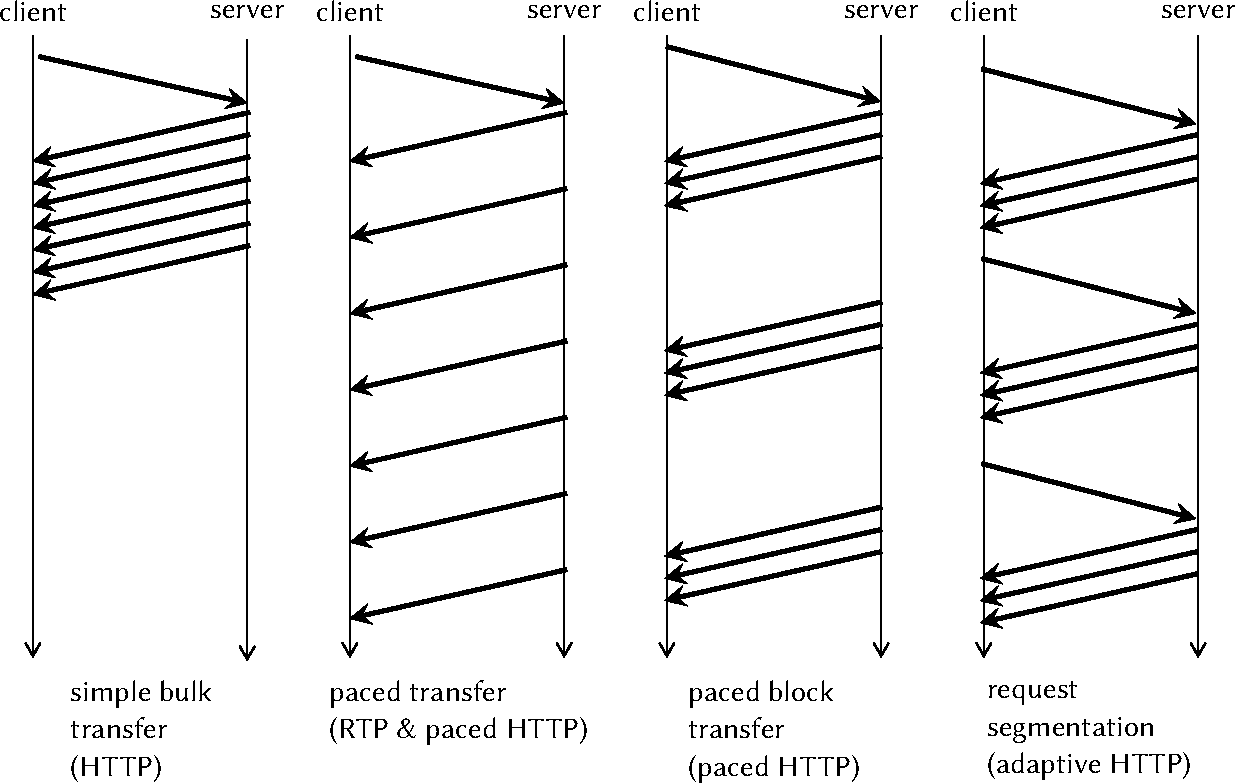
\includegraphics[width=1.0\textwidth]{images/streaming-transfer-modes.pdf}
\caption{Comparison of several possible streaming transfer modes \cite{ma2011mobile}.}
\label{c3:fig:streamingtransfermodes}
\end{figure}

\todo{reference to transmission pattern here? alternatively, put one of the old youtube throttling pictures here}

The first of the alternatives to achieve control over the playback buffer using \gls{HTTP}-streaming is to appropriately size \gls{TCP}'s flow control receive window by the application. 
Alternatively, the \gls{HTTP}-server can also manually throttle the download process, through various pacing strategies. The second and third transmission diagrams in Figure~\ref{c3:fig:streamingtransfermodes} depict two possible strategies compared to a regular \gls{HTTP} file transmission in the first transmission diagram. A third way, is to either partition the stream file into smaller even-spaced segments, that have to be requested independently, or use the aforementioned range requests on the stream's file. Through this, the receiving application can delay the request of new ranges or segments so that it matches a targeted bitrate over a longer timeframe.

These mechanism, however, can also result in a very bursty block-like transmission, a so-called ON-OFF pattern, and can cause undesirably interactions with \gls{TCP}'s flow and congestion control mechanisms \todo{ref to interaction}. Overall, stretching out the transmission may reduce server load spikes and the required buffer size on the client device but also makes streaming more vulnerable to insufficient network \gls{QoS} parameters. These specific approaches to pace to a target rate can generally be subsumed under the term \textit{Application Layer Flow Control}, which is also being implemented by some Web streaming services, e.g. YouTube \cite{alcock2011afcyt,metzger2011delivery}.

The aforementioned only adapt the transmission rate to the stream's bit rate and not the stream rate itself. Different video bitrates may be desired for many use cases, especially reacting to changing network conditions, take vertical handover from a 802.11 to a \gls{UMTS} network with a much lower throughput as an example. Quality adaptation with \gls{HTTP} streaming is generally achieved through the described range request or file segmentation mechanisms. For both approaches, multiple versions of the file or the segments have to be generated in different encoding quality levels. Also, the video file format needs to be able to support switching the stream and have an index to correlate the video files with their quality level and temporal position. \cite{ma2011mobile, watching-video1}

Several formal adaptive streaming protocols are in the process of standardization. \gls{HLS} \cite{pantos2011livestreaming} defines a playlist format to be stored separately on a server that links to all available stream variants and segments thereof in sequence. \gls{DASH} \cite{Stockhammer:2011:DAS:1943552.1943572} is a \gls{ISO}/\gls{IEC} \cite{iso-iec-23009-1} and 3GP-DASH \cite{3gpp.26.247} standard. Herein, all video segments are gathered in an alternative XML-based presentation scheme. Due to its file-based, using \gls{HTTP} for streaming is much more suited for stored video. But has also been successfully employed for live content, both \gls{HLS} as well as \gls{DASH} support this.


HTTP includes some support by the network in the form of proxies, but there are signaling methods that can e.g. forbid the caching of specific content through the no-cache directive \cite{rfc2616}.



\paragraph{Multicast}

No multicast, but can use CDN to almost the same effect.
	On the other hand, the rise of community pages like YouTube has shown, that the interest does not lie in watching the same content at the same time, but rather in high individualism. Therefore, multicast is less relevant for today's streaming. If there is a media event that is streamed live, one can always fall back to using the relatively new structures of \gls{CDN} to be able to serve large groups of users while still conserving bandwidth on the Internet backbones.


WebSocket\footnote{\url{http://www.websocket.org/}} \cite{ietf2011websocket} is a protocol running atop of \gls{HTTP} offering connection multiplexing and asynchronous as well as full duplex communication. It could be used to implement a more flexible \gls{HTTP} video streaming offering or unlocking further use cases. Similar approaches should be included and evaluated in the research for this thesis.

By using \gls{HTTP} the ideal platform for the client is either a plugin living inside a Web browser, the method chosen by Flash, or the browser itself, that in most cases has built-in video playback capabilities.

Location of Control: client-side and in-band ... but with websockets and SPDY / HTTP/2.0 could also be server side through server push

The capabilities and shortcomings of these novel mechanisms are not yet fully researched making it one of the prime foci of the thesis. Of special interest are:



%% <-- WIP




%%%%%%%%%%%%%%%%%%%%%%%%%%%%%%%%%%%%%%%%%%%%%%%%%%%%%%%%%%%%%%%%%%%%%%%%%%%%%%%%
\subsubsection{Other and Proprietary Approaches}

RTMP, ...

There are also other proprietary and standardized streaming systems which better fulfill the requirements of specific fields of applications. \gls{MBMS} \cite{3gpp22.146,3gpp22.246} is a specification defined by the 3GPP group for multicasting multimedia traffic specific to the architecture in mobile networks. But similar to \gls{RTP} the number of implementations and their acceptance are negligible.

The explicit control structure of protocol suites like \gls{IMS} \cite{3gpp.23.228} and \gls{MBMS} weaves application and network layer tightly together. This theoretically allows for an improved streaming performance at the cost of universally applicable behavior.

Peer-to-peer based approaches, including live-streaming!; describe P2P, 

%%

\begin{table}[htbp]
  \caption{Protocol Classification Matrix.}
  \label{c3:tab:streamingclassification}
  \tabulinesep=1.2mm
  \centering
  \begin{tabu}{|X|X|X|X|X|X|} 

  Protocol & \textbf{Location of Control} & \textbf{Reliable Transport} & \textbf{Video Type} & \textbf{Adaptivity} & \textbf{Multicast} \\ \tabucline[1pt]-\everyrow{\tabucline[on 1.5pt off 2pt] - }
  RTP &  &  &  & & \\
  simple HTTP & & & & & \\
  adaptive HTTP (DASH) & & & & & \\
  RTMP &  &  &  & &
  \end{tabu}
\end{table}


%% <-- %% end WIP
%%

%%%%%%%%%%%%%%%%%%%%%%%%%%%%%%%%%%%%%%%%%%%%%%%%%%%%%%%%%%%%%%%%%%%%%%%%%%%%%%%%
\subsubsection{Network Stack Layers and Streaming}
\label{sec:analysis}

In network layering models, it is often assumed that the layers are independent (or at least strongly decoupled) from, and only present narrow interfaces to, one another. From a conceptual point of view, media streaming is a process governing the application layer. Thus, the application and its behavior might be thought to dominate the overall streaming process and associated quality. In this Section, we will show that this is not necessarily the case.

Figure \ref{c3:fig:timescales} overviews the approximate time scales on which activities on different layers may take place, spanning a remarkable range of twelve orders of magnitude. Multiple layers might implement the same or similar functionality, e.g. flow control in the application and on transport layer, resulting in nested control loops, which might be coupled due to the timing constraints. 

\begin{figure}[htbp]
	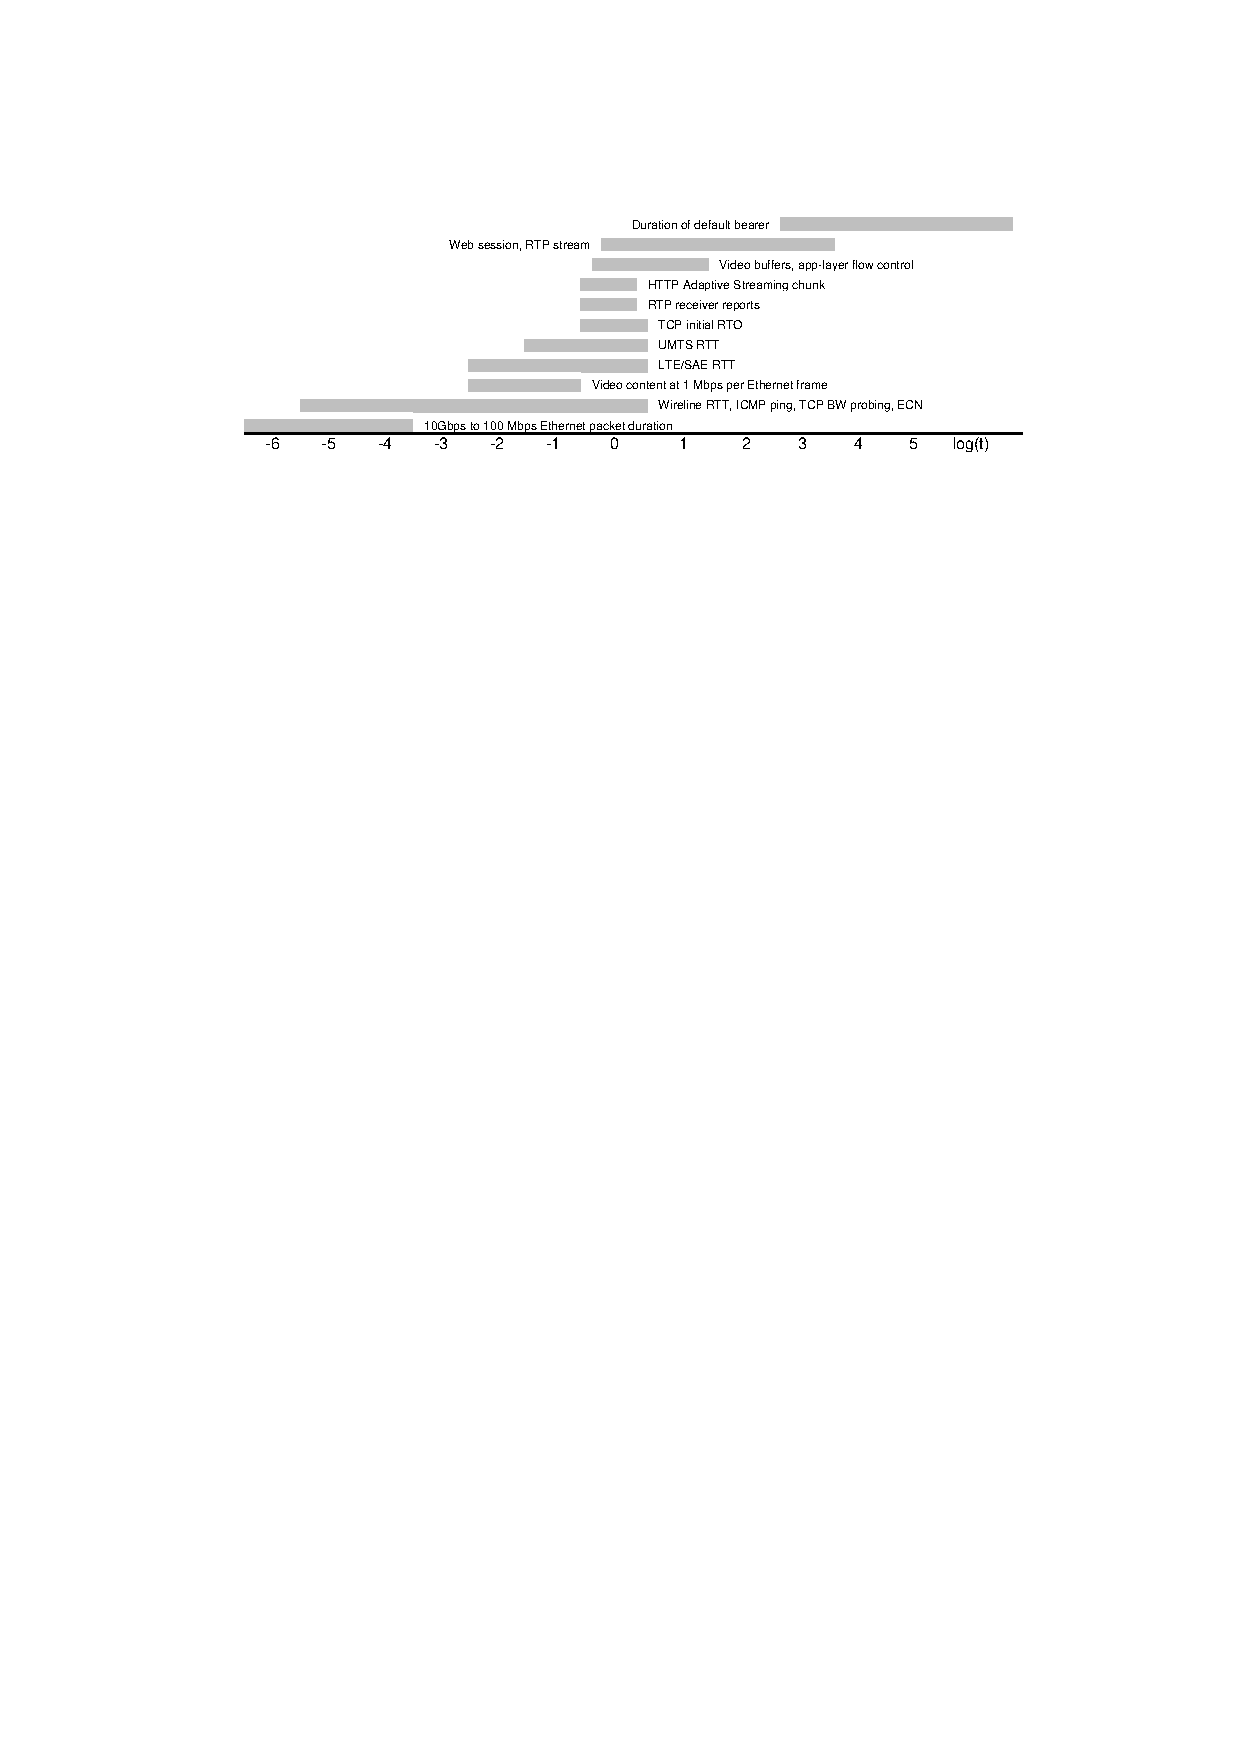
\includegraphics[width=\textwidth]{images/timescales.pdf}
	\caption{Relevant time scales in the layers of the stack}
	\label{c3:fig:timescales}
\end{figure}


\subsubsection{Network Layer}

As seen in Figure \ref{c3:fig:timescales}, the time constants found in different network implementations range from nanoseconds (for Gigabit Ethernet) to seconds (for UMTS and \gls{LTE}/\gls{SAE} wireless networks), depending on the technology used. This also influences the achievable round-trip time across such networks, which directly affects the performance of higher-layer protocols: \gls{IP}, \gls{ICMP}, \gls{UDP}, \gls{TCP}, and subsequently all application-layer protocols are all subject to these timing constraints.

In the case of wireless networks, typical effects of wireless connectivity relating to physical phenomena like fading and interference come into play. Flaky radio connectivity is a major source of packet loss and excessive delay. Certain cellular mobile technologies like \gls{UMTS} and its evolutions implement loss concealment themselves, confounding IP's assumption of a host-to-network layer lacking guaranteed delivery. Other peculiarities of cellular mobile networks include a \gls{MTU} opaque to IP, and delay variances as functions of packet sizes \cite{Arlos10} and radio access technologies \cite{laner2011dissecting}.


 Then, the technological progress enables both handsets and the network to become faster: Comparing the delay budgets given by x for \gls{UMTS} (2005) and y for \gls{HSDPA} R99 (2009) respectively, it is seen that the delay caused by processing on the mobile terminals decreased by a factor of 30, and that the core network has become faster by an order of magnitude as well. \cite{svoboda2006composition} has additional information on the delay budgets per network entity, varying the packet size as the parameter.
\gls{LTE} and \gls{SAE} also makes heavy use of the concept of bearers, a type of tunnel through the mobile network associated with quality levels and policy control. Although the bearer concept already exists in \gls{UMTS}, operators seem cautious to configure other bearers than the default one, and support by hand-sets is not widespread either. The setup procedure of \gls{LTE} bearers is sufficiently lengthy to be measurable and influence packet delay on initiating connections. 
\todo{re-insert references}
%
For reasons of radio spectrum efficiency, applications with long patterns of inactivity may be scheduled to not use HSDPA. This also causes measurable additional delay for applications [SVOB and their references 3 and 4].
%


\subsubsection{Transport Layer}

The two most widely used transport protocols are \gls{TCP} and \gls{UDP}. As is widely known, \gls{TCP} implements a number of elaborate mechanisms to establish and tear down connections, deliver data to the application in sequential order, conceal loss on the network layer, adapt its bandwidth usage to the capabilities of the other endpoint (flow control) and the network (congestion control), and share bandwidth fairly through a distributed control algorithm. Furthermore, its notion of ports adds a layer of addresses on top of the network layer.

UDP also supports port numbers, but does not include any of the other mechanisms \gls{TCP} has. This spurs the common misconception that \gls{UDP} is the faster transport protocol. In fact, all packet types are subject to the same round-trip time, independent of the transport protocol used. Delays in the delivery of data to the upper layer occur in \gls{TCP} when segments are considered lost in transmission (via timeouts or gaps in the range of acknowledged segments). \gls{TCP} retransmits the lost segments, causing the round-trip time to spike temporarily. In the case of \gls{UDP}, the application layer handles (or ignores) packet loss.

As indicated in the previously, mobile cellular networks often conceal packet loss, which is used by TCP as an indication for network congestion. Rather than lost, packets are highly delayed, which can cause sub-optimal bandwidth usage. Mobile networks also show artifacts relating to port and network address translation (commonly subsumed under \gls{NAT}), firewalling, and middleboxes interfering with \gls{TCP} timeout on long-lived connections \cite{sigcomm11middleboxes}.

\subsubsection{Application Layer}

There exists a diversity of streaming applications and associated application-layer protocols, each supporting to differing degrees certain types of streaming, and each having its own set of requirements, depending on the content type (pre-generated or live), the codec and its bitrate, and playback control and quality feedback.

One classification for streaming protocols might be their body of standardization: There are many proprietary protocols with undisclosed or legally restricted standards documents, e.g. \gls{RTMP}, \gls{MMS}, and \gls{WMSP}. Other protocols and protocol families are standardized by open bodies such as the \gls{IETF} In our work, we focus on these ``open'' protocols.

In the latter category are two well-known protocol families for media streaming, \gls{RTP} and \gls{HTTP}. \gls{RTP} sees most of its use in walled garden services such as IP TV. HTTP is the single most common application layer protocol on the Internet, owing its popularity to the ubiquity of web browsers. As \gls{RTP} is designed for media transport, a companion protocol suite consisting of \gls{RTCP} (for control information), \gls{RTSP} (for stream control like pausing), and \gls{SDP} (for session management) is often used. \gls{RTP} is mostly transported using \gls{UDP}.

In contrast to \gls{RTP}, \gls{HTTP} was not designed for specific payload types apart from \gls{HTML}. The actual streaming protocol behavior is defined by the application, not by the protocol. Every service is thus free to define its own distinct protocol behavior. For \gls{HTTP}, many de-facto variants for streaming exist, but many if not most are not formally standardized. There is work underway in the \gls{IETF} to create a standard for \gls{DASH}.



Within these protocol families, a multitude of implementations exist that suit specific demands. \gls{RTP} specifies an initial set of profiles (RFC3551 \cite{rfc3551}), with a multitude of definitions cropping up with every new type of media coding scheme . In HTTP, the actual transfer model, addressing, and metadata mechanisms have been in place virtually unchanged since 1999, when HTTP/1.1 was specified. Much innovation has since gone into the payloads transferred via HTTP, as well as the control of its underlying transport protocol, TCP.

Both protocol families offer a wide range of techniques, established and recent, de-facto and formally standardized, each supporting different types of streaming and content, and each subject to the interplay of content requirements, the application, the network, the media player, the layer stack, etc. Seemingly, not one single protocol can solve all problems at once. 

The Real-time Transport Protocol (RTP) \cite{rfc3550} is an IETF protocol designed for (near) real-time payload such as multimedia or sensor data. It is designed for support by the network. \gls{RTP} supports mixers and translators that enable transcoding of content as it travels through the network.

Since RTP is typically transported over UDP, it is also multi-cast compatible. For example, A1 Telekom Austria’s A1TV uses an Organization-local cope Multi-cast \cite{rfc2365} tree with distinct IP addresses for each program. At the same time, \gls{UDP} is not inherently congestion-controlled, and \gls{RTP}'s own congestion control mechanism (if activated at all) has a relatively long delay to respond for reasons of rate limiting on the control channel. This means a wide-spread use of \gls{RTP} could even cause congestion collapses in parts of the network.



\subsubsection{Protocol Comparison}
In \gls{RTP} streaming, it is customary to have multiple flows for different parts of the media stream, e.g. audio and video, and a separate control connection. In \gls{HTTP}, one (or multiple consecutive) TCP connection is used for both control and data transfer.
In \gls{RTP}, flow control on the transport layer needs to be done by the server application. The same goes for congestion control, which is implemented using receiver reports, or might be left out altogether. HTTP uses TCP as its transport protocol, and thus inherits its flow control and congestion control features.
There are several implementations for application-layer flow control. Simple bulk transport is the typical web download model, which assumes that both the client and the server try to transfer the data as fast as possible. Contrarily, paced transfer is implemented by \gls{RTP}, where the server sets the bitrate the client will see. An interesting variant on paced transfer is paced block transfer, implemented for example in the YouTube block sending mechanism. The specific incarnation consists of server-controlled burst sending of 64kB blocks and inter-block gaps of variable length to adjust the download rate to the average video bitrate. An additional initial burst phase is present to prefill buffer.
 
Playback control is actually done by the server in the case of RTP, where the client issues requests to, e.g., pause the stream, and the server then reacts. In HTTP, the client is in much stronger control of the playback, and need not notify the server of a user's decision to skip backwards, etc. 
For the exchange of transport control information such as packet loss, RTP uses a companion protocol named \gls{RTCP}. HTTP again leverages TCP, where such information is exchanged implicitly. It must be noted however that due to the flexible data format RTCP pro-vides, more concise information can be signaled in addition to transport control related matters.
To conclude, the different protocols are also specified to different degrees. As stated before, there is a large body of \glspl{RFC} relating to RTP and its adaption to new media, content, etc. For HTTP, many de-facto used variants adapted to streaming exist, but many if not most are not formally standardized. There is work underway in the \gls{IETF} to create a standard for \gls{DASH}.



% \begin{figure}[htbp]
% \centering
% 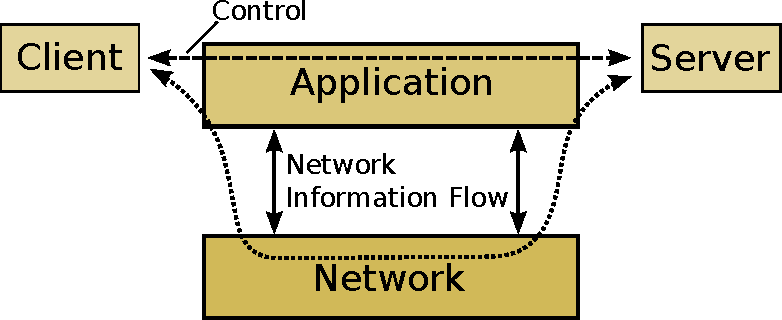
\includegraphics[width=0.8\textwidth]{images/nif.pdf}
% \caption{Theoretical information exchange paths between streaming partners.}
% \label{c3:fig:nif}
% \end{figure}

%One future trend is said to be an increase in the required communication confidentiality and authentication. One of the goals might be to enable full end-to-end encryption on the transport level of the network. This could be achieved either by providing an encrypting alternative to TCP, e.g. CurveCP \cite{curvecpwww} and TCPCrypt \cite{tcpcrypt}, or by using HTTPS and moving other functionality further up the stack.


% \subsubsection{Video Delivery Architecture}
% \label{c3:sec:videodeliveryarchitecture}
% Large Internet sites are not hosted at one central site anymore, but are usually served through geographically distributed entities forming a load-balancing structure. Such load balancing mechanisms have a long history on the Web, e.g. in the form of mirror servers a user can select manually.

% In today's Content Distribution Networks (CDN), a much larger number of mirror servers is available, and selection of a server is no longer carried out explicitly by the user, but implicitly through DNS: Content is addressed using URLs (\texttt{http://somedomain/somepath} in its simplest form), and the CDN's DNS servers are configured to resolve certain domain names to different IP addresses, depending on where the query originated.

% To get an insight into the structure of YouTube's content distribution network, we undertook a two-step measurement campaign \cite{rafetseder2011explyt}. First, we downloaded and manually parsed the HTML code served by YouTube's web servers. We could thus enumerate and learn about the structure of domain names in the system. The most relevant category of domain names for our purposes takes the form of \texttt{v$\alpha$.lscache$\beta$.c.youtube.com}, where $0<\alpha<25$ and $0<\beta<9$. Not all permutations of names are found at all times. We also noted that there are hostnames that seem to point to geographical locations, but have not succeeded so far in exhaustively mapping those two types of names.

% The second part of our campaign consisted of active measurements on forty distributed computers (part of the \textit{Seattle} Internet testbed\footnote{\url{https://seattle.poly.edu/html/}} \cite{Cappos:2009:SPE:1508865.1508905}) for over 600 hours. We learned that the frontend web server name, \texttt{www.youtube.com}, resolves to multiple IP addresses per geographical location of the probing host which are mostly disjoint from sets of addresses found on other hosts. The number of frontend IP addresses also changes over time, e.g. to account for load variations such as load increases during the evening hours in the hosts' time zones. The actual video cache servers only have one IP address per name and location each, but sometime this address is seen to change during the day. 

% When looking at the resolved addresses per frontend server and time zone, two interesting time-dependent scaling effects can be seen: First, servers become reachable or vanish in a coordinated manner controlled by the time of day, i.e. in a 24 hour pattern. We speculate this provides a gain in efficiency for the overall system to turn on parts of the resource pool for load balancing only when there is demand.

% The second type of effect occurs much more seldom. It stretches out over multiple days and is best described as follows: A new block of server IP addresses is made available in addition to the existing ones. After a few days of parallel operation, a previously active block is taken out of service. The new block continues to serve. Comparison measurements  performed in parallel show that this switch-over between IP address blocks has a positive effect on the latency to the servers, as the latency to non-YouTube destinations show no improvements at all.

%%%%%%%%%%%%%%%%%%%%%%%%%%%%%%%%%%%%%%%%%%%%%%%%%%%%%%%%%%%%%%%%%%%%%%%%%%%%%%%%
%!TEX root = ../../dissertation.tex
%%%%%%%%%%%%%%%%%%%%%%%%%%%%%%%%%%%%%%%%%%%%%%%%%%%%%%%%%%%%%%%%%%%%%%%%%%%%%%%%
\section{Related Work}
\label{c4:sec:relwork}

The investigations conducted in both this and the subsequent chapter do not fall strictly into an existing research category but instead aim to provide diverse insights into the control plane from the perspective of the core network. Nonetheless, a selection of publications from the tackled fields is collected here and the interesting aspects for this work are noted. In the following sections the related work is divided into four distinct fields.

Work in the first and second sections evaluate properties of the mobile network and its traffic. They are distinguished in their approach to the investigation, as the first group uses active measurements from mobile devices or conclude from other sources of traffic whereas to the other one has access to passive measurements from inside a \gls{3G} mobile network. Publications from the third category can be generally subsumed under the term \textit{traffic modeling} and may not be specific to cellular networks. The final field concerns itself with investigative work conducted by the responsible standardization and organizational bodies themselves, i.e., the \gls{3GPP} and \gls{GSMA}.


%%
\subsection{Device Active Measurement Investigations}

The approach taken by active measurement studies is simple yet still very insightful. They are performed by writing custom application layer measurement programs for a mobile device. Specific traffic patterns are then generated, recorded, and evaluated. While this can provide very detailed information about the higher network layers, it is limited both in lower layer information as well as scale, due to being limited to a rather low number of devices.

Despite being more or less completely specified in the \gls{3GPP} documents, there is no open layer 1 and 2 (together also called ``baseband'') implementation for \gls{3G}.\footnote{Apart from OsmocomBB (\url{http://bb.osmocom.org/trac/}), but it only provides \gls{GSM} and partial \gls{GPRS} functionality.} Therefore, the baseband's behavior can not be directly instrumented from the application layer. Attempts to infer some properties are still worth conducting as the following selection of publication demonstrates.

In~\cite{Xu:2011:CDN:2007116.2007149} Xu et al.\ use data from a location service combined with active measurements to determine the possible geographic location of a \gls{GGSN} in order to improve the location of application content caches for the current network infrastructure. Similarly, in \cite{sigcomm11middleboxes} Wang et al.\ developed a program to probe mobile networks for middle boxes. That term includes any node, that alters traffic and affects performance not intended by the actual end-to-end protocols. Examples are \gls{CGN}~\cite{rfc7021}, firewalls, or intercepting \gls{HTTP} proxies. A large number of such nodes were present in the investigated mobile networks and resulted in increased device power usage and download durations and even pose security issues themselves.

Concerning methods to infer specific baseband and \gls{RRC} state machine timer values with active measurements, a 2007 paper~\cite{4640935} presents a way to do this by transmitting packets with a varying inter-departure time and studying the resulting arrival pattern. Indeed, the dynamics of the radio interface's \gls{RRC} signaling and involved state machines are under investigation by several publications. However, almost all focus solely on the impact at the radio interface but pay little attention to potential implications in the \gls{CN}.

The aforementioned work is continued in \cite{5360763} and uses the presented tools to derive \gls{RRC} transitions and power usage from traffic patterns. They found, that operators have a rather larger freedom in configuring the mobile network control plane state machines and deviate from the standard and even omit some states completely.

A further example of cross-layer influences in mobile cellular networks is \cite{qian2011profiling}. It discusses the impact of application layer behavior on \gls{RRC} signaling and its consequences for device energy consumption and radio channel allocation efficiency. The authors argue that there is much room for improvement in this area, and propose some enhancements.

This is further elaborated on by research from Schwartz et al.\cite{schwartz2013angrybirds} using the same technique to analyze the radio signaling load and thus power efficiency from several mobile phone applications. The impact of custom set state machine timers interacting with application traffic is further investigated and the \gls{QoE} is investigated.


%%
\subsection{Research Based On Network Traces}

The second alternative to mobile network investigations comes in the form of recording and evaluation traffic traces inside the network. This brings a much larger experiment scale with it, albeit usually at the cost of some finer grained details in the higher protocol layers because of aggregation to flow level. With core network measurements, the signaling traffic of the observed link can also be directly investigated, which is a huge benefit compared to the guesswork in active measurements.

The authors of \cite{4675847} investigate the influence of individual \gls{CN} nodes on the one-way delay distribution of user traffic packets. According to the work, the latency portion added by the \gls{SGSN} is larger but also fluctuating more, while the \gls{GGSN} added a small but steady amount of latency. This provides us with initial clues on the expected load impact of the \gls{CN} for the investigations in this work.

Following up on the topic of mobile network one-way delays is Laner~et~al.\ in \cite{laner2012delaycomparison}. The end-to-end latency of an early \gls{LTE}/\gls{EPC} network implementation is compared to that of a \gls{HSPA} network at several measurement points in the networks. The results show a lower median latency for \gls{LTE}, despite some scenarios still being in favor of \gls{3G} networks.

The authors of \cite{Shafiq:2012:FLC:2254756.2254767} limit their focus to a specific subset of connected devices, namely those of \gls{M2M} type. These are small automated devices, that periodically send out data, e.g., sensor readings, or receive control commands. The paper attempts to characterize these on the basis of their generated mobile network traffic. The patterns are clearly distinguishable from traffic caused by other device types such as smartphones.

A 2012 publication~\cite{Zhang:2012:UCC:2377677.2377764} presents us with a more general look on the traffic composition of cellular access networks in comparison to wired access network. Much more and shorter flows are occurring in the case of cellular networks. It will be interesting to see if this shorter-but-more theme is also evident in signaling traffic. Additionally, even traffic pattern distinctions between types of applications are made showing a wide range of possible outcomes across the investigated applications.

Both the authors of \cite{shafiq2011characterizing} and \cite{paul2011understanding} take the approach of looking at high-level user traffic characteristics in a mobile network, focusing on temporal and spatial variations of user traffic volume and peeking at the influence of different devices on this metric. Additionally, \cite{baer2011two} delivers a theoretical introduction on how to conduct large scale network measurements and compares some data evaluation approaches. The 2008 paper of \cite{4570772} takes a look at times scales and time of day deviations observed in aggregated user traffic in a mobile network.

Up until now no trace-based investigation considered the control plane in their evaluation. The following publications include this at least to some degree.

In 2006, Svoboda~et~al.~\cite{svoboda2006composition} conducted a core network measurement study of various user traffic related patterns, and also provided an initial insight into \gls{PDP} context activity and durations. Another paper~\cite{lee2007detection} combines simulations based on WiFi and synthetic traces with prior knowledge of \gls{RRC} states and their effects to investigate detection methods for signaling \gls{DDoS} occurring on the radio interface. A possible magnitude of this type of attack is discussed. This also gives an indication of the correlation between user traffic patterns and radio signaling.

A 2010 publication\cite{Qian:2010:CRR:1879141.1879159} uses the indirect \gls{RRC} inferring method described earlier on a core network \gls{TCP} trace data set and finds that the involved \gls{RRC} state machine is largely inefficient in terms of signaling overhead and the device's energy consumption for the traffic patterns seen in the data. 

A more recent publication at \cite{he2012panoramic} performs a \gls{RRC} investigation at the path between \gls{RNC} and \gls{SGSN}. The authors classify their evaluations based on device model and vendor and on the application type, and find that different devices have strongly different \gls{RRC} characteristics, which could possibly also have an impact on \gls{gtp} signaling. Here, the \gls{RRC} evaluation was done in a direct manner using explicit logs from the \gls{RNC}. A final paper~\cite{Ricciato2010551} recaps some general attack scenarios on \gls{3G} networks that exploit the specific \gls{3GPP} system design. These are often closely related to the control plane.


%%
\subsection{Traffic Modeling}

Extracting viable models from mobile traffic measurements will also play a significant role. The first related work is a survey of source modeling approaches for \gls{GPRS} user traffic from the year 2000 \cite{staehle2000source}. Models for \gls{HTTP} traffic and user behavior are compared and a combined model is recommended. One has to keep in mind, though, that due to the rapid developments in the Web in recent years those models might no longer be valid. 

Similarly, the authors of \cite{965876} derive a synthetic \gls{UMTS} traffic model from wired dial-up traces. By using a batch Markovian arrival process they characterize session traffic in most cases with a lognormal distribution.

Work conducted in \cite{Halepovic:2005:CMU:1089803.1089969} derives a model for the users' mobility in a mobile network. The mobility model is however more focused on the circuit-switched voice communication features of a phone. Likewise, the authors of \cite{Pesch2005385} introduce a traffic model for \gls{SIP} \gls{VoIP} communication in \gls{UMTS} networks. However, this model is specific to the \gls{IMS} domain of \gls{UMTS} and potentially not applicable to the more common over-the-top pure \gls{SIP} traffic. But the model additionally investigates some initial \gls{UMTS} control plane timing values, such as the processing time of \gls{PDP} context activation messages.

A further publication in 2005 \cite{Landman200568} attempts to model the delay of \gls{IP} packets passing through an \gls{UMTS} network using a batch Markovian arrival process. However, the model specifically focuses solely on the delay originating from processing at the radio link and not at the core nodes.

Finally, a further paper by Laner~et~al.~\cite{6214330} investigates, amongst other things, a user's session duration and throughput in a \gls{HSDPA} network. The duration is modeled as an exponential distributions and the throughput using a lognormal distribution, albeit both exhibit additional heavy tail characteristics.


%%
\subsection{\texorpdfstring{\acrshort{3GPP}}{3GPP} and \texorpdfstring{\acrshort{GSMA}}{GSMA} Related Work}

The two associations related to the mobile network under scrutiny, the \gls{3GPP} as well as the \gls{GSMA} themselves have also released some studies and recommendations concerning potential effects of and issues with the control plane. 

In reaction to the mentioned \gls{RRC} signaling \gls{DDoS} the \gls{GSMA} released some best practices \cite{gsma2011fdbestpract} intended to reduce the number of signaling messages in these circumstances. The cause of the \gls{DDoS} were in most cases mobile devices, that circumvented the \gls{RRC} state transition timers and explicitly switched the radio to the idle state after a transmission was finished and re-enables it whenever needed. This can greatly reduce the power usage but increases the number of signaling messages to be sent and thus the load in the radio network and possibly also inside the \gls{CN}. With the presented ``Fast Dormancy'' mechanism, mobile devices are supposed to reduce the radio signaling amount while still saving energy. The implications of this mechanism on the core are not investigated.

A \gls{3GPP}-released study \cite{3gpp.22.801} also describes the diverse traffic mix originating from modern smartphones and its associated signaling problems.

The aim of the study in \gls{TS}~23.843~\cite{3gpp.23.843} is to document some of the control plane bottlenecks and attack vectors on the \gls{CN}. This also includes the interesting case of \gls{GTP-C} overload and causes for this scenario. Some approaches to alleviate the effects are also presented but mostly targeted at the \gls{EPC}. The final study is an extension to the last one \cite{3gpp.29.807} and focuses solely on \gls{GTP-C} overload control to be included in a future version of the \gls{3GPP} architecture. Therefore, the mostly unfinished document again targets just at a future version of \gls{LTE} and provides no investigation of the actual load situation in current \gls{3G} networks.

All of the presented publications relate to some degree to this chapter. However, the combination of the aspects of \gls{CN} signaling with a statistical evaluation and load modeling of \gls{PDP} contexts should be a genuine contribution of this chapter.



%24.826 \cite{3gpp.24.826} Study on impacts on signalling between User Equipment (UE) and core network from energy saving; deals mostly with switching off cells and moving over UEs, not actual core network efficiency



%%%%%%%%%%%%%%%%%%%%%%%%%%%%%%%%%%%%%%%%%%%%%%%%%%%%%%%%%%%%%%%%%%%%%%%%%%%%%%%%
\section{Metrics for Reliable Transport Streaming}
\label{c3:metrics}

%% <-- WIP

%% <-- %% end WIP

Quality Estimation and Modeling: QoE metrics, MOS, stalling time and buffering models, subjective and objective testing

%%%%%%%%%%%%%%%%%%%%%%%%%%%%%%%%%%%%%%%%%%%%%%%%%%%%%%%%%%%%%%%%%%%%%%%%%%%%%%%%
\subsection{Unreliable Streaming Metrics}
... and why they mostly do not work / are not applicable.



%%%%%%%%%%%%%%%%%%%%%%%%%%%%%%%%%%%%%%%%%%%%%%%%%%%%%%%%%%%%%%%%%%%%%%%%%%%%%%%%
%!TEX root = ../../dissertation.tex
%%%%%%%%%%%%%%%%%%%%%%%%%%%%%%%%%%%%%%%%%%%%%%%%%%%%%%%%%%%%%%%%%%%%%%%%%%%%%%%%
\section{Streaming Modeling}
\label{c3:sec:modeling}

As stated, the goal of this chapter is to model the measuring process and reliable streaming. This section will introduce our reliable \gls{TCP}-based streaming model. It is intended for easily comparing different protocol variants against each other and measuring all variants in one testbed. 

But first, because any evaluation of a model requires metrics, we describe ones appropriate to the model and give a rationale.
 
%%%%%%%%%%%%%%%%%%%%%%%%%%%%%%%%%%%%%%%%%%%%%%%%%%%%%%%%%%%%%%%%%%%%%%%%%%%%%%%%
\subsection{Metrics for Reliable Transport Streaming}
\label{c3:metrics}

When measuring anything related to video or even just image quality, one has the choice between conducting a subjective or objective assessment. 

During a subjective test, human assessors evaluate and rate video quality in a controlled environment with the results usually being aggregated into an overall relative quality score \gls{MOS}. Through the human element, conducting a subjective assessment is very time and resource consuming but it also achieves the highest precision.

This is where, objective video quality assessments come into play. Modern objective models attempt to recreate the features of the humans' visual perception and psychophysics and are calibrated by subjective assessments. Most objective models operate on a full reference approach, they directly compare the original reference video to the resulting video after being encoding or transmitted.

Two of the simplest full reference image quality metrics, which can also be applied on video, are the \gls{MSE} and \gls{PSNR}, defined as:

\begin{equation}
    \begin{aligned}
    MSE = \frac{1}{N} \sum_{i=1}^{N}(x_i - y_i)^2\\
    \text{and } PSNR = 10 \log_{10} \frac{L^2}{MSE},
    \end{aligned}
\end{equation}

with $N$ as the number of pixels in a frame and individual pixels $x$ and $y$ from the reference and output frame respectively. $L$ denotes the maximum value of a pixel. For grayscale or when investigating each color channel separately, usually $L = \SI{8}{\bit} = 255$.  \cite{objective-vqa}

Image quality models can by nature only test for spatial distortions of a single image. This includes a general blockiness or blurriness, noise, or reduced resolution. Dedicated video quality assessments can additionally take temporal metrics into account, e.g. frame rate anomalies. Such models are being researched and standardized by the \gls{ITU} and \gls{VQEG} for example in \cite{ituJ144, ituJ246, ituJ247}.


When conducting dedicated streaming quality measurements, only this portion should be taken into account by a metric, and not the initial encoding process. During streaming only a specific subset of quality degradations can occur. Lost or late packets can cause missing blocks in a frame or frames to be skipped completely. Initial thoughts concerning \gls{IPTV} \gls{QoE} have been given in \cite{ituG1080} and the influence of packet delay variations on playout buffers is investigated in \cite{rfc3393}The \gls{MDI} \cite{rfc4445} is an attempt to capture this behavior and relate it to the network \gls{QoS}. Its metric relies on two properties, the \gls{DF}, as a measure of the network's latency and jitter, and the media loss rate. Of special interest to this investigation is the \gls{DF}, which is calculated based on a virtual buffer (VB) of received stream data as

\begin{equation}
    \begin{aligned}
        VB = r_{rcv} - r_{drain} \\
        DF_i = \frac{\max(VB) - \min(VB)}{r_{drain}}
    \end{aligned}
\end{equation}
 
Reliable streaming has even less possibilities to degrade a video stream. Packets can not be out of order and loss is concealed by \gls{TCP}, meaning that the transmitted and the played video are identical. The only thing that can still happen, is portions of the video arriving too late to be played out at their intended point in time.
A potential reliable streaming quality assessment metric needs to keep track of the following properties:

\begin{itemize}
    \item The initial delay, which is the time delta between the start of the transmission and the start of the video play.
    \item The number and lengths of interruptions or stalls during playback.
    \item For adaptive streaming, the characteristics of the quality levels the video was played in. This includes the number of switching events and the duration of each level.
\end{itemize}

A concise metric covering all properties has not been defined yet. The \gls{CI} was defined in \cite{1498486} and used to determine quality in \gls{P2P} live streaming. It is defined as \enquote{the number of segments that arrive before or on playback deadlines over the total number of segments} and with this partly captures the stalling property. In \cite{5634160} and \cite{DBLP:journals/corr/SeyedebrahimiBP13} a so-called \gls{PI} is defined and evaluated. The definition $I_p = uv$ is simply based on the number of stalls $u$ and the average stall duration $v$. 

Generally, most research operates just directly on these three properties, which allows for the most freedom in usage scenarios. The streaming measurement model presented in the following section also works with the assumption, that only the three properties are of importance. The model assumes no special metric, the individual properties can be directly attained from the model. Though any metric could still be applied on the results.


%%%%%%%%%%%%%%%%%%%%%%%%%%%%%%%%%%%%%%%%%%%%%%%%%%%%%%%%%%%%%%%%%%%%%%%%%%%%%%%%
\subsection{Measurement and Playback Model}
\label{c3:model}

Parts of the model presentation is based on the author's previous work published in \cite{cs3518}, \cite{metzger2011delivery}, and \cite{6229739}. It is based on the desire to compare all in-the-wild variants of reliable streaming protocols in a simple and concise way. This is achieved by basing the model on the component that is common to all of the approaches: the playback buffer.

To display a video stream, an application needs to maintain a playback buffer of sufficient size to at least gather enough data to reconstruct one single atomic unit of playback such as a video frame.
From the perspective of a player application , a video consists of a sequence of atomic units, video frames and audio samples.
The application progressively decodes the video from a source and stores the units temporarily in a memory buffer before playing them. In reliable streaming, the buffer is filled by the payload from received \gls{TCP} segments a subject to the network \gls{QoS}. The process can be subsumed as:

\begin{equation*}
\mathit{buffer}(t) = \sum_{0}^{t} \text{data}_\mathrm{received} - \sum_{0}^{t} \text{data}_\mathrm{played}
\end{equation*}

Both the incoming and outgoing data stream are variable over time. The fill level of the playback buffer is the critical component in the playback process and the central element of the model.If the buffer reaches a size of zero the playback process stops and stalling occurs.

\begin{figure}[htb]
    \centering
    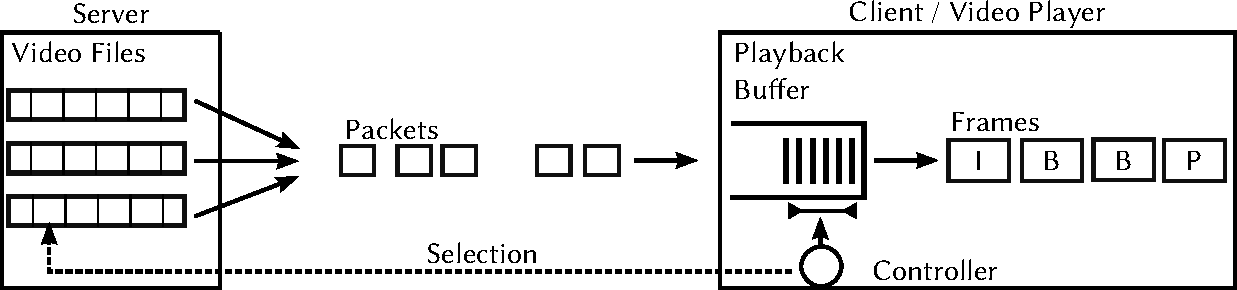
\includegraphics[width=0.9\textwidth]{images/playback-model.pdf}
    \caption{Reliable streaming playback model based on buffer control.}
    \label{c3:fig:playback-model}
\end{figure}

Figure~\ref{c3:fig:playback-model} overviews the reliable streaming model. The controller, part of the video player, selects a video from a remote location and the transmission is started, filling the playback buffer. The model has three degrees of freedom, which are all governed by the controller and together are coined playback strategies. These are:

\begin{itemize}
    \item The initial playback delay, which is the time between the initiation of the video stream transmission and the actual stream playback. The larger this is chosen, the bigger the safety margin on the buffer gets. If the video and transmission bitrate are known to be constant and and appropriately dimensioned, the initial delay can be chosen to be very small.
    \item Playback pause and resume decisions based on the current buffer fill level. This is a generalization of the initial playback delay, which is in fact only one, albeit always occurring stalling period.
    \item Selection of the video or video segment with a video bitrate chosen according to the current network throughput. This is only applicable for adaptive streaming.
\end{itemize}


These decisions yield a stalling period distribution for a streamed video. The frequency and the duration of stalls directly relate to the decision function of the playback model. The more frequent the stalls are, the shorter they will be; if the strategy produces longer stalls, they will be less frequent assuming the same network conditions. The time scale on which streaming applications buffer content usually lies in the range of seconds. This is a necessity in best-effort networks, as the available network bitrate might drop unexpectedly and cause stalling.


The the rest of this sections present fundamental playback strategies and strategy building blocks with features extracted from real world examples, which are given afterwards. 



%%
\subsubsection{Null Strategy}

The simplest strategy is having no strategy at all. Playback is started immediately when at least a single frame fully resides within the buffer and stops again at an empty buffer. The behavior can be summarized as ``Whenever anything can be played from the buffer, do so''.

This results in frequent stops and a large loss in playback continuity and will therefore not be used in practice. However, this strategy has some interesting theoretical properties, which is why it is mentioned here.
It minimizes total stalling time and the required buffer space. Moreover, it gives an upper limit for the number of stalls occurring\footnote{As a video frame is atomic, no other model could possibly stop the playback more often.}. Therefore, it can act as a baseline reference to assess the performance of other strategies.

\begin{figure}[htb]
    \centering
    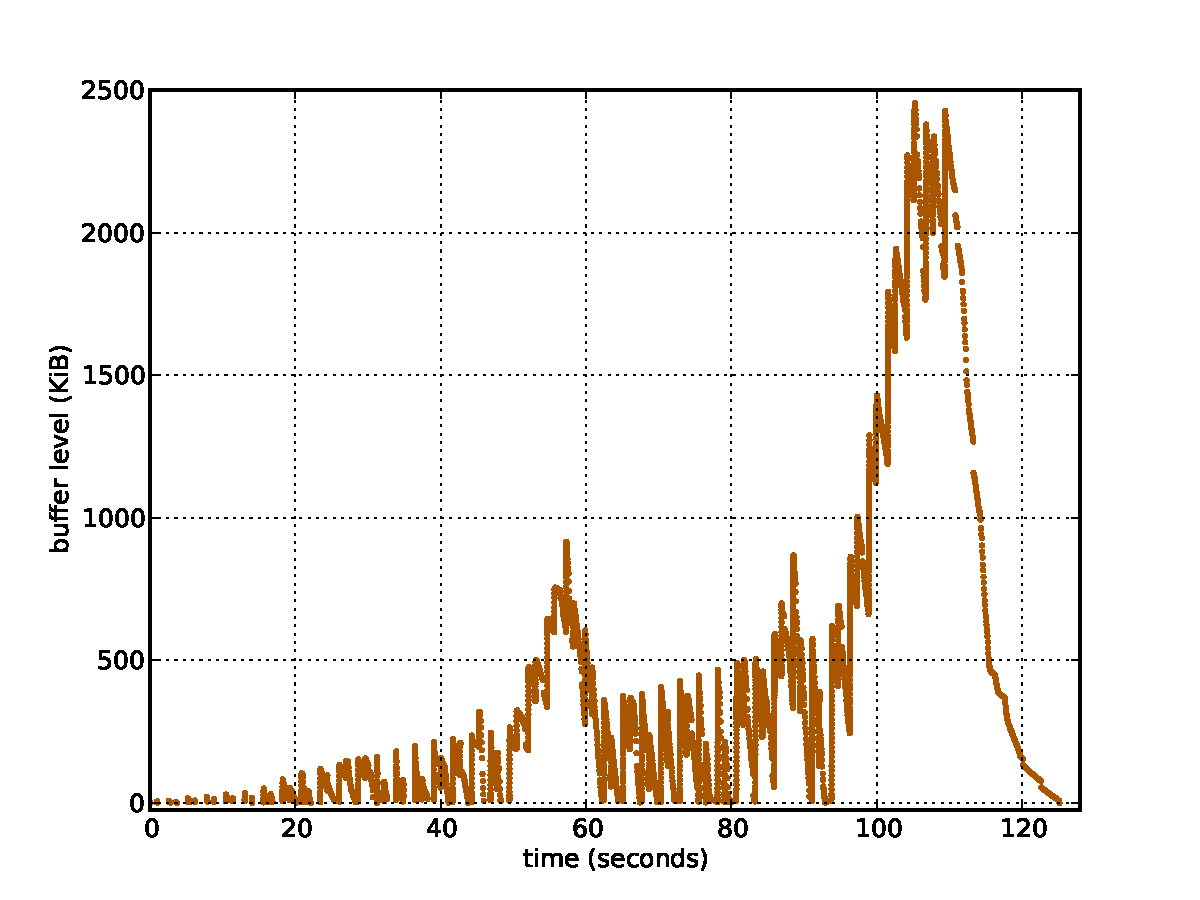
\includegraphics[width=0.9\textwidth]{images/bufferlevel-stall-new.pdf}
    \caption{Buffer fill level with null strategy; \SI{33}{\second} total stalling.}
    \label{c3:fig:bufferlevel-stall}
\end{figure}

Figure~\ref{c3:fig:bufferlevel-stall} depicts an exemplary time series diagram of the contents of a video buffer using this strategy with a transmission rate only slightly above the video stream's rate. The buffer frequently drops down to zero forcing a short stall. According to the presented related work on the \gls{QoE} impact of stalling frequency in comparison to the length of stalls \cite{6123395}, this is the worst possible scenario for a person watching the stream.


%%
\subsubsection{Threshold Strategies}

Instead of instantly restarting playback, a lower threshold can be introduced. Only after a certain buffer fill level threshold has been surpassed, playback will be started. Thresholds can be set independently for the initial playback delay and stalls, with the initial playback delay generally set to be higher.

The threshold can be chosen in a number of ways. It can either be an absolute data volume, a buffered video duration. The latter is much more suited for variable bitrate videos as it automatically adapts itself to the current bitrate. A third option is to buffer for a certain amount of real time -- this can be seen as threshold -- and starting playback after that period regardless of the volume of the buffer. Additionally, the threshold could also either be set to a constant value or dynamically chosen according to the expected network \gls{QoS}.

Besides this single-threshold strategy, a two-threshold strategy might make more sense for segment-based streaming. In addition to the lower threshold, an upper threshold is introduced. When reached, no new segments will be requested until the buffer arrives at the lower threshold again.  To achieve an hysteresis effect a third threshold, somewhere between the lower and upper bound, can also be introduced. Through this, the maximum buffer size can also be controlled. This is important in situations with hard limits on available memory. Mobile devices come to mind here.

\begin{figure}[htb]
    \centering
    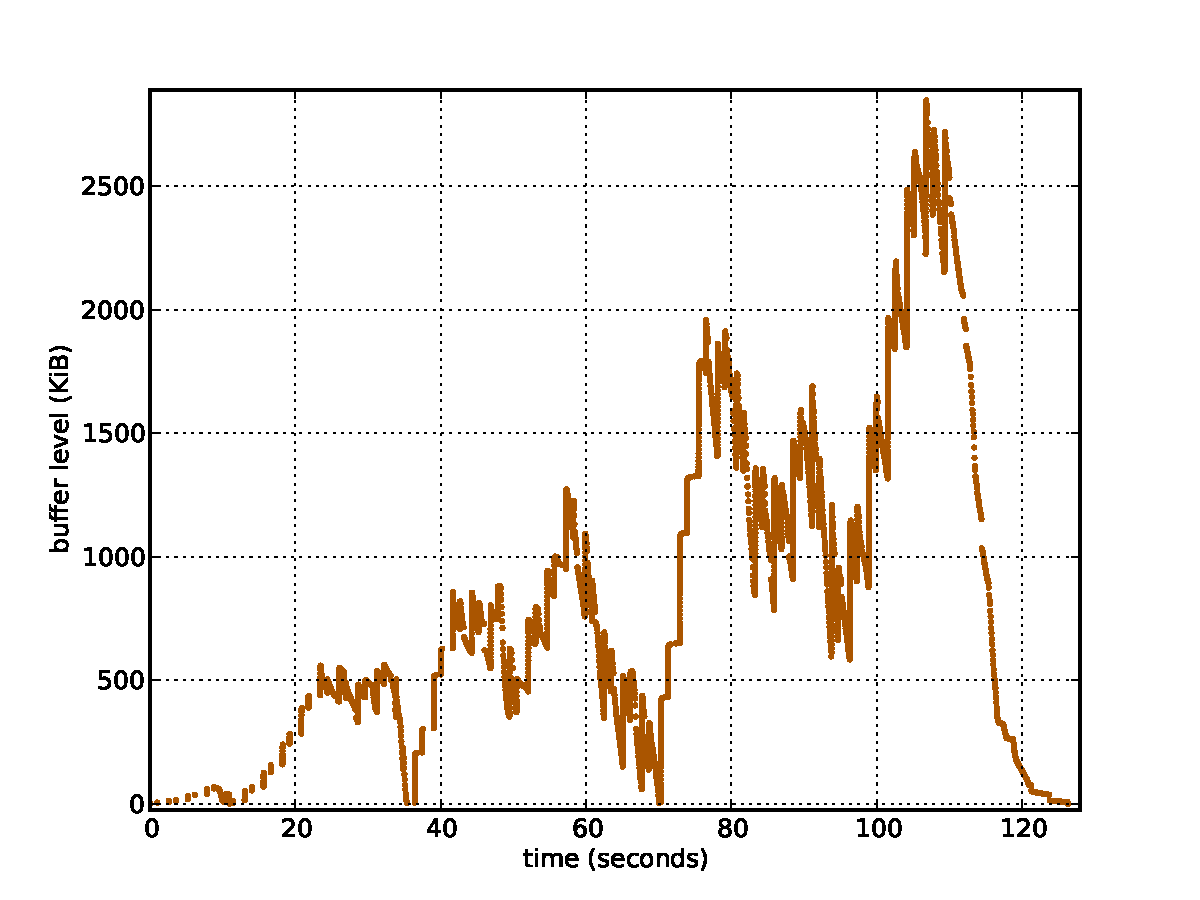
\includegraphics[width=0.9\textwidth]{images/bufferlevel-flash-new.pdf}
    \caption{Sample buffer fill level for a \SI{2}{\second} and \SI{5}{\second} buffered video duration threshold strategy; \SI{34}{\second} total stalling.}
    \label{c3:fig:bufferlevel-flash}
\end{figure}

An example buffer diagram is displayed in Figure~\ref{c3:fig:bufferlevel-flash}. In this case, the initial delay was controlled by a buffered video duration threshold of \SI{2}{\second} and a resume condition also based on buffered video duration but with a \SI{5}{\second} threshold. The strategy produces noticeable less stalls than the null strategy but slightly increases the total stalling time.


%%
\subsubsection{Pacing Strategies}

For segment-based \gls{HTTP} streaming, a two-threshold strategy is not the only supplemental option on top of simple streaming. Here, the controller can pace the request of future segments to match the overall, or the current video bitrate. A safety margin can also be factored in to even out short time fluctuations of either the transmission or the video bitrate. For example, the controller would request segments with an overall transmission rate of 1.25 times the video bitrate. The pacing rate can either be statically chosen in advance or can be calculated dynamically based on current or future conditions. The latter leads to predictive strategies.

%%
\subsubsection{Predictive Strategies}

In predictive strategies, knowledge of the future of the streaming process is used by the controller to adjust the start/stop and segment retrieval conditions. Instead of global knowledge, heuristics can instead attempt to approximate a future state.

A very simple predictive approach is to prolong the initial delay to the point, that no intermediate buffer underrun and thus no stall will occur. With global knowledge, the controller can start the stream at the earliest possible point in time, thus minimizing the total stalling time while still having only the initial delay.

\begin{figure}[htb]
    \centering
    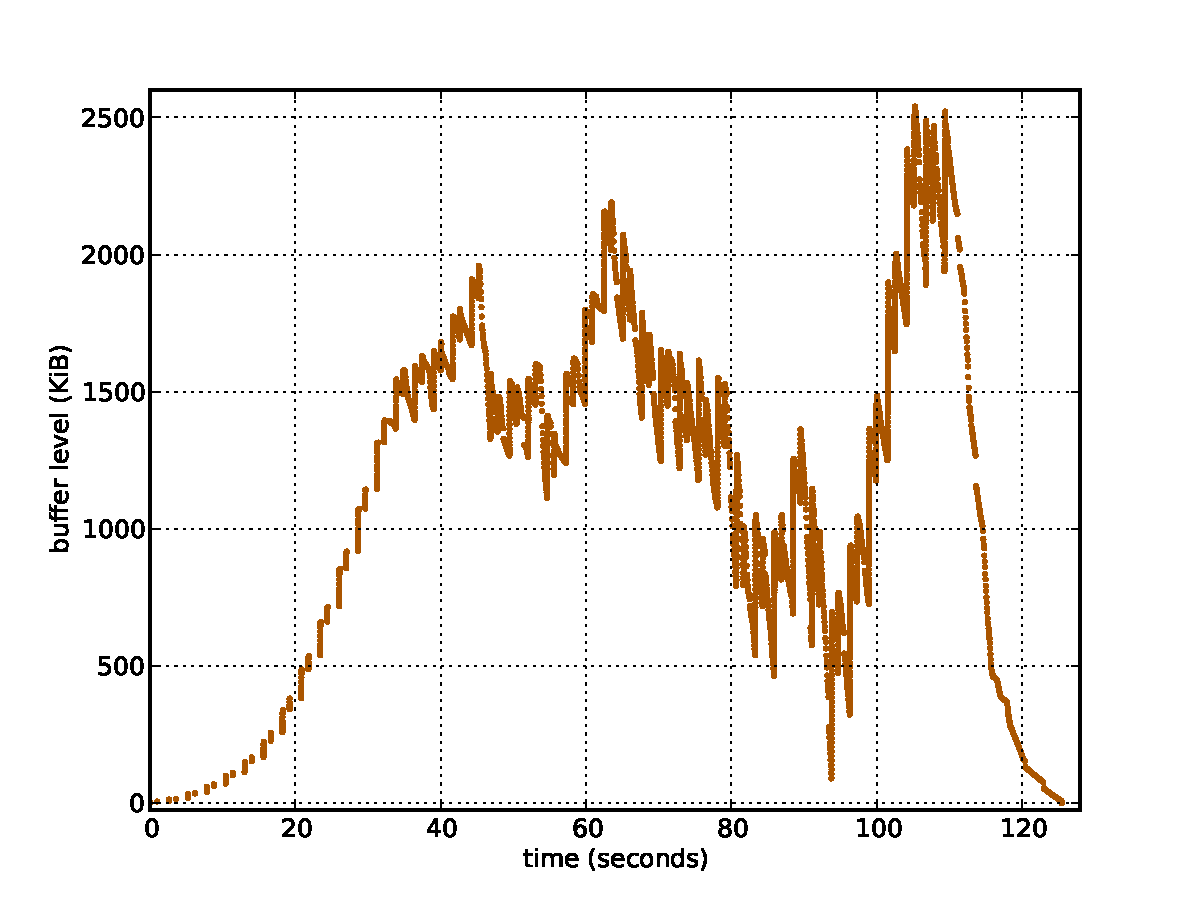
\includegraphics[width=0.9\textwidth]{images/bufferlevel-startdelay-new.pdf}
    \caption{Sample Buffer fill level for the delayed playback model, \SI{33}{\second} total stalling.}
    \label{c3:fig:bufferlevel-startdelay}
\end{figure}

Figure~\ref{c3:fig:bufferlevel-startdelay} depicts the time series of a sample implementation of this delayed playback predictive strategy with all necessary stalling occurring upfront.


%%
\subsubsection{Adaptive Strategies}

Most strategies for adaptive streaming are an extension of both the threshold as well as the pacing strategy. However, instead of a simple transmit-or-no-transmit ruleset, they can make much more fine-grained adjustments. The quality of the stream segment to be requested will be chosen, depending on the current fill level and drain rate of the buffer. This makes a trade off between maintaining a certain quality level and putting up with increased waiting times, and dropping the quality to a level sustainable at the current transmission rate.


\subsubsection{Real World Implementation Examples}

Actual streaming player implementations often do not implement only one of these strategies, but rather combine ideas from several. Herein, thresholds are often set arbitrarily through the implementor's best practices and not empirically evaluated, often making a trade-off between user perceivable quality and resulting server load. In general, every streaming service practically implements its own playback strategies. This section describes three example applications.

%%
\paragraph{2011 YouTube Flash Player Buffering Strategy}

Google's video streaming site YouTube is constantly changing its appearance and technical makeup. In recent years, YouTube streams are delivered by one of three players: The Website's Flash player, a browser-integrated HTML5-based player, or custom player implementations in mobile phones, set-top boxes and similar devices. Here, the Flash-based variant used in 2011 is described.

This player used a single threshold strategy with different threshold values for the initial delay and any subsequent stalls. The values were already described in Figure~\ref{c3:fig:bufferlevel-flash}. This model assumes sufficient network conditions in the beginning, requiring only a short initial playback delay to pre-fill the playback buffer. If, however, stalling occurs, then it will buffer longer to keep the stalling frequency down.

\begin{table}[htb]
    % increase table row spacing, adjust to taste
    %\renewcommand{\arraystretch}{1.3}
    \caption{Transmission Related Parameters from YouTube's Video URL Setup}
    \label{c3:tbl:yturl}
    \centering
    \begin{tabu}{|X[l]|X[p]|}
        \hline
        URL Part & Description \\ \hline
        \texttt{v$\alpha$.lscache$\beta$.c.youtube.com} &  Cache server involved in the delivery.\\
        \texttt{algorithm=throttle-factor} and \texttt{burst=40} and \texttt{factor=1.25} & Indicates initial burst plus block sending configuration. \\
        \texttt{ratebypass=yes} & Parameter to indicate no rate limiting.\\ \hline
    \end{tabu}
\end{table}

Furthermore, YouTube employs a proprietary pacing mechanism outside of the control of the streaming player. This is hinted at in the encoding of the \glspl{URL} of the video files and enforced by the video file cache server. Some of those not user-changeable parameters are described in Table~\ref{c3:tbl:yturl}. The pacing was in effect for all videos below high definition resolution, but has since then been extended to include all video files. 

\begin{figure}[htbp]
% used yt-delay/hPUGNCIozp0_delay_100 2, spyder with matplotlib config patch
    \centering
        \begin{subfigure}[b]{0.90\textwidth}
                \centering
                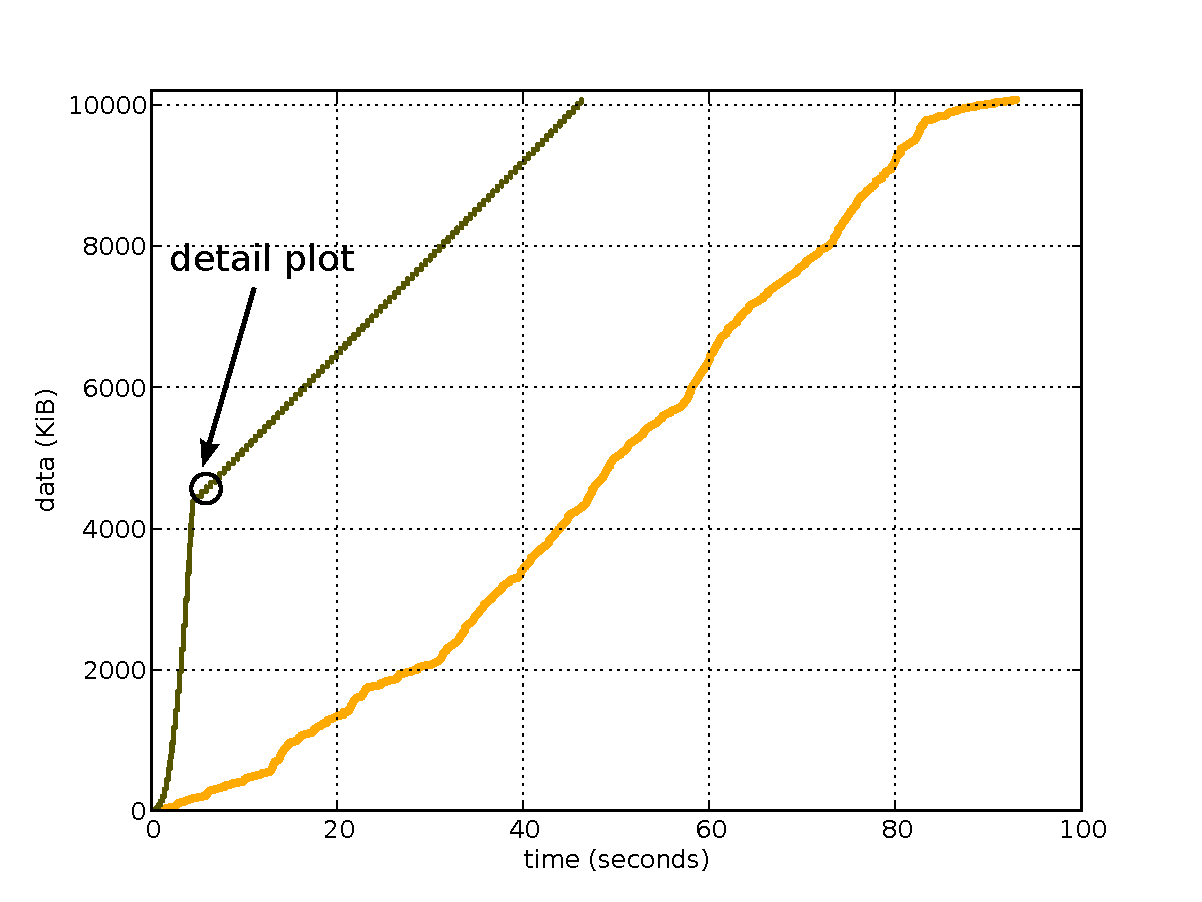
\includegraphics[width=\textwidth]{images/blocktransfer-mod.pdf}
                \caption{Overall graph.}
                \label{c3:fig:blocktransfer-overall}
        \end{subfigure}

        \begin{subfigure}[b]{0.90\textwidth}
                \centering
                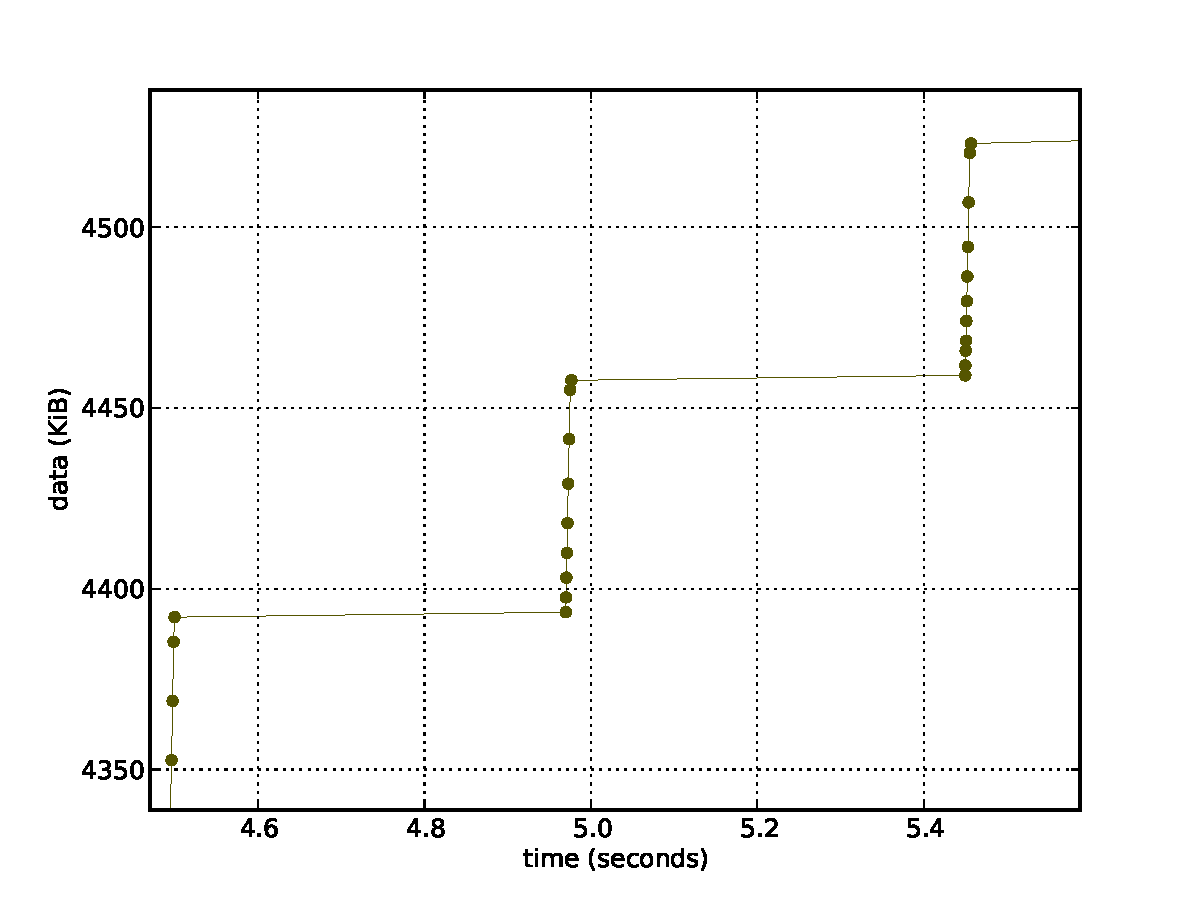
\includegraphics[width=\textwidth]{images/blocktransferdetail.pdf}
                \caption{Detail plot of the rate-limited block-sending phase.}
                \label{c3:fig:blocktransfer-detail}
        \end{subfigure}
\caption{Comparison of downloaded and consumed data volume revealing the pacing mechanism used by YouTube.}
\label{c3:fig:blocktransfer}
\end{figure}


The throttling method, also observed in \cite{alcock2011afcyt}, limits the transmission to a rate slightly above the average media bitrate, measurements and the \gls{URL} scheme indicates this to be a factor of the video bitrate of $1.25$. The rate limit is not constant, instead a ON-OFF block-sending scheme is facilitated. The scheme transmits short packet bursts, typically \SI{64}{\kibi\byte} in size, followed by long pauses as seen in Figure~\ref{c3:fig:blocktransfer}. The pause length between two bursts is set dynamically to reach the targeted bitrate on a larger time scale. The initial phase of the stream transmission is conducted unthrottled at line speed, presumably to allow for some pre-buffering to occur at the client media player. A possible reason for this server-side pacing is to avoid load spikes, with the added side effect of keeping the clients' buffer sizes in check.



%%
\paragraph{Firefox's HTML5 Player Strategy}

Video streaming can also be directly conducted with the Web browser, through the use of a HTML5 canvas element. The \gls{W3C} specifies the default technical process of HTMl5 video streaming in \cite{html5video} and essentially suggests a predictive strategy. Herein, the Web browser should estimate and correlate the transmission rate to the video bitrate. A property called ``autoplay'' uses this definition to start  playback of the associated video \enquote{as soon as it can do so without stopping}. The HTML5 strategy also allows to limit the buffer size through transmission pacing, negotiated with the server, and appropriately timed range requests.

The open-source Firefox browser represents an implementation of this specification and substantiates it further. The description of this strategy is based on Firefox's version 4.0 released in March 2011. Because it is an online algorithm which does not have global knowledge of the video and transmission speeds of any point in the future it has to estimate these.
To estimate the current and future rates, the moving average of the transmission rate $s_{MA}$ and the video bitrate $v_{MA}$ are calculated. The condition $c$ Firefox uses to start and resume the playback process is given in Algorithm~\ref{c3:alg:firefox}, with the buffered video duration $b_b$, and the duration spent buffering $b_T$.

\begin{algorithm}[htb]
    \centering
    \begin{algorithmic}
        \IF {$s_{MA} > v_{MA}$} 
          \STATE $c \gets ( b_b=20s \lor b_T=20s )$
        \ELSE
          \STATE $c \gets ( b_b=30s \lor b_T=30s )$
        \ENDIF 
    \end{algorithmic}
    \caption{Firefox playback (re-)start decision algorithm.}
    \label{c3:alg:firefox}
\end{algorithm}

 \begin{figure}[htb]
    \centering
    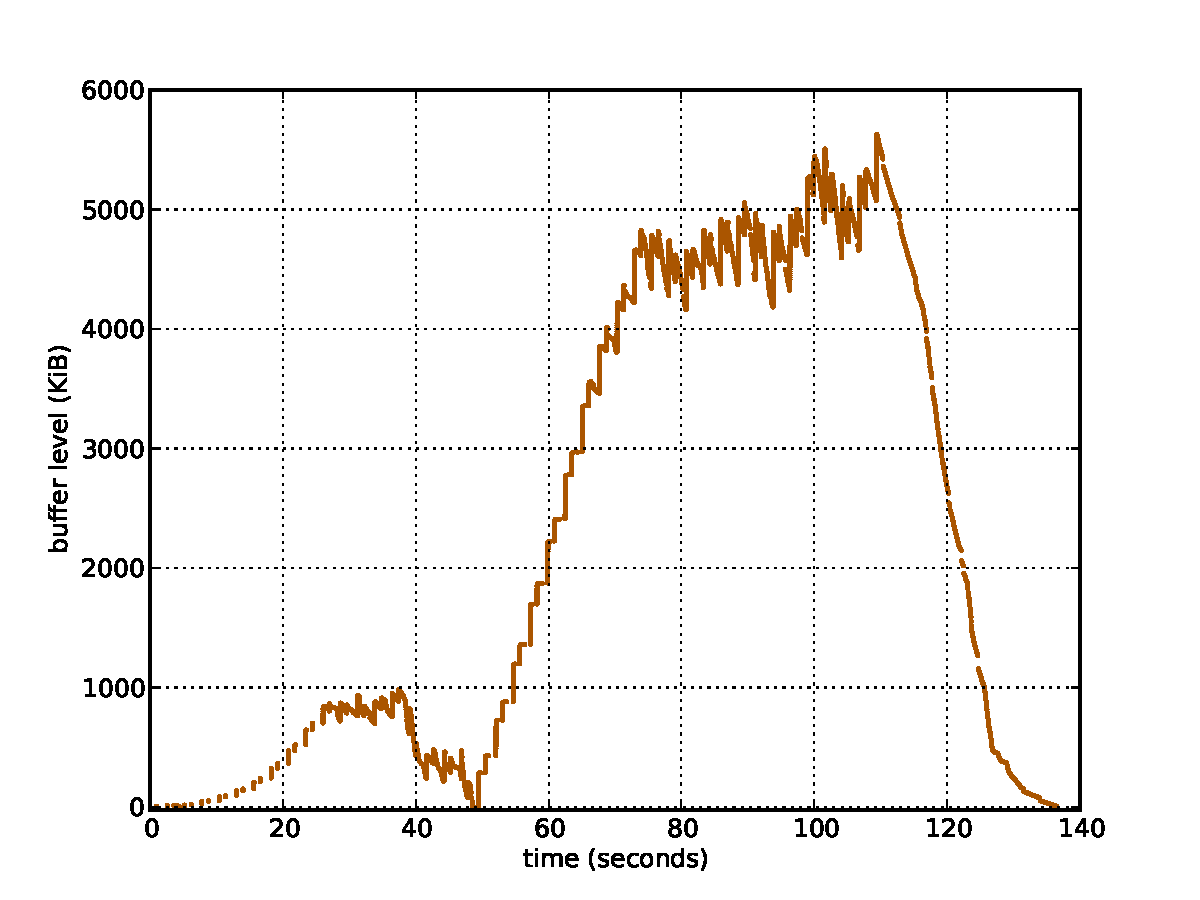
\includegraphics[width=0.9\textwidth]{images/bufferlevel-firefox-new.pdf}
    \caption{Sample buffer fill level for the Firefox 4 strategy, \SI{44}{\second} total stalling.}
    \label{c3:fig:bufferlevel-firefox}
\end{figure}


This approach is quite conservative and trades off long stalling periods for fewer stalls. The test case for our model is shown in Figure \ref{c3:fig:bufferlevel-firefox}. The playback starts only after a long waiting period and intermittent stalls cause a long buffering period. 
Due to the longer overall stalling time the player needs to buffer more data than other strategies. This may make it unsuitable for devices with sparse amounts of memory, e.g. mobile phones. On the other hand, could a large buffer also increase the chance of continuous playback in such scenarios with bad \gls{QoS}.


\paragraph{Adaptive streaming strategies}

Implementations for adaptive streaming players are again mostly proprietary and their behavior has to be derived from measurements. This is even true for adaptive streaming protocols, which have open specifications as these generally do not specify the player's behavior.

Microsoft's Silverlight player's strategy is described in \cite{BLTJ:BLTJ20505}. It employs a two-threshold model and rate estimations. When on of the thresholds is reached, the quality will be adjusted by one step upwards or downwards as long as the transmission rate is sufficient.

The buffering behavior of further protocol variants, including Adobe's \gls{HTTP} Dynamic Streaming, Apple's \gls{HTTP} Live Streaming and a sample implementation of \gls{DASH}, are investigated in \cite{Muller:2012:EDA:2151677.2151686,akhshabi2011experimental}.




% \begin{itemize}
% \item The player has been buffering data for at least 30 seconds.
% \item The player has already buffered an amount of data corresponding to 30 seconds of video.
% \item The video download has been completed.
% \item The moving average of the transmission rate is larger than the moving average of the video bitrate and the player has a safety buffer with 20 seconds of video data.
% \end{itemize}

% \begin{table}[htb]
%     \caption{Variables involved in buffering decisions.}
%     \label{c3:tbl:buffvars}
%     \centering
%     \begin{tabu}{|l|X[p]|} 
%     \hline
%     Variable & Description \\ \hline
%     $s_{MA}$ & Moving average of the transmission speed. \\
%     $v_{MA}$ & Moving average of the video bitrate. \\ 
%     $c$   & Condition upon which to start/resume playback. \\
%     $b_b$    & Amount of video data the buffer contains. \\
%     $b_T$    & Amount of time spent in non-playing buffering state. \\ \hline
%     \end{tabu}
% \end{table}

% used yt-delay/hPUGNCIozp0_delay_2500 1, spyder, color #aa5500
% data
% start delay 33s 
% flash 33.82s
% stalling 32.68s
% html5 as implemented in firefox 44s


%Which offers better quality to users? Some approaches (TODO: refs and explain how)

% Longer waiting time but very few stops. Stalling model definitely the shortest waiting time but stops too frequent with insufficient network conditions, i.e. can not really be used. Delayed playback requires total knowledge not available beforehand. Can maybe used with reduced information, bandwidth estimation, but this is essentially HTML5/Firefox.




%``application comfort'' time to skip, ...
%\subsubsection{Unreliable Streaming Metrics}
%... and why they mostly do not work / are not applicable.


%%%%%%%%%%%%%%%%%%%%%%%%%%%%%%%%%%%%%%%%%%%%%%%%%%%%%%%%%%%%%%%%%%%%%%%%%%%%%%%%
%!TEX root = ../../dissertation.tex
%%%%%%%%%%%%%%%%%%%%%%%%%%%%%%%%%%%%%%%%%%%%%%%%%%%%%%%%%%%%%%%%%%%%%%%%%%%%%%%%
\section{Measurements}
\label{c3:sec:measurements}

With these playback models at hand, this section demonstrates how to conduct actual evaluations of reliable streaming protocols with it.

As discussed, there are numerous incarnations of reliable streaming protocols in use. Almost all of them follow the same basic approach but with slight variations in execution and choice of playback strategies and corresponding parameters. But it is exactly these choices that can have a large impact on the streaming process and resulting quality. 

The problem lies in comparing these protocols to each other. Each of them is usually tied to a specific --- and most often proprietary closed source --- streaming player. Setting up all these players in one testbed is a huge effort and requires very specific software environments to be used on the client machines. Moreover, these players are built with user interaction and not automation and directly measuring the outcome in mind. This can still be achieved through extensive workarounds, but must be tailored to every player application. The presented approach avoids this hassle and provides a concise way to test any conceivable playback strategy in one single test setup.


%%
\subsection{Progressive Streaming Measurement Framework}

To enable quick evaluations for progressive streaming the framework follows a two phase approach, separating the active online recording phase from the passive playback emulation. Recording data is very time intensive and cannot be sped up when conducting investigation of a real world process, and not relying on simulated data. It still replicates the steps a user would perform to consume a media stream on a playback device. Through appropriate configuration different scenarios can be modeled, e.g. network conditions, behavior and specifics of the user device.
 
\begin{figure}[htb]
    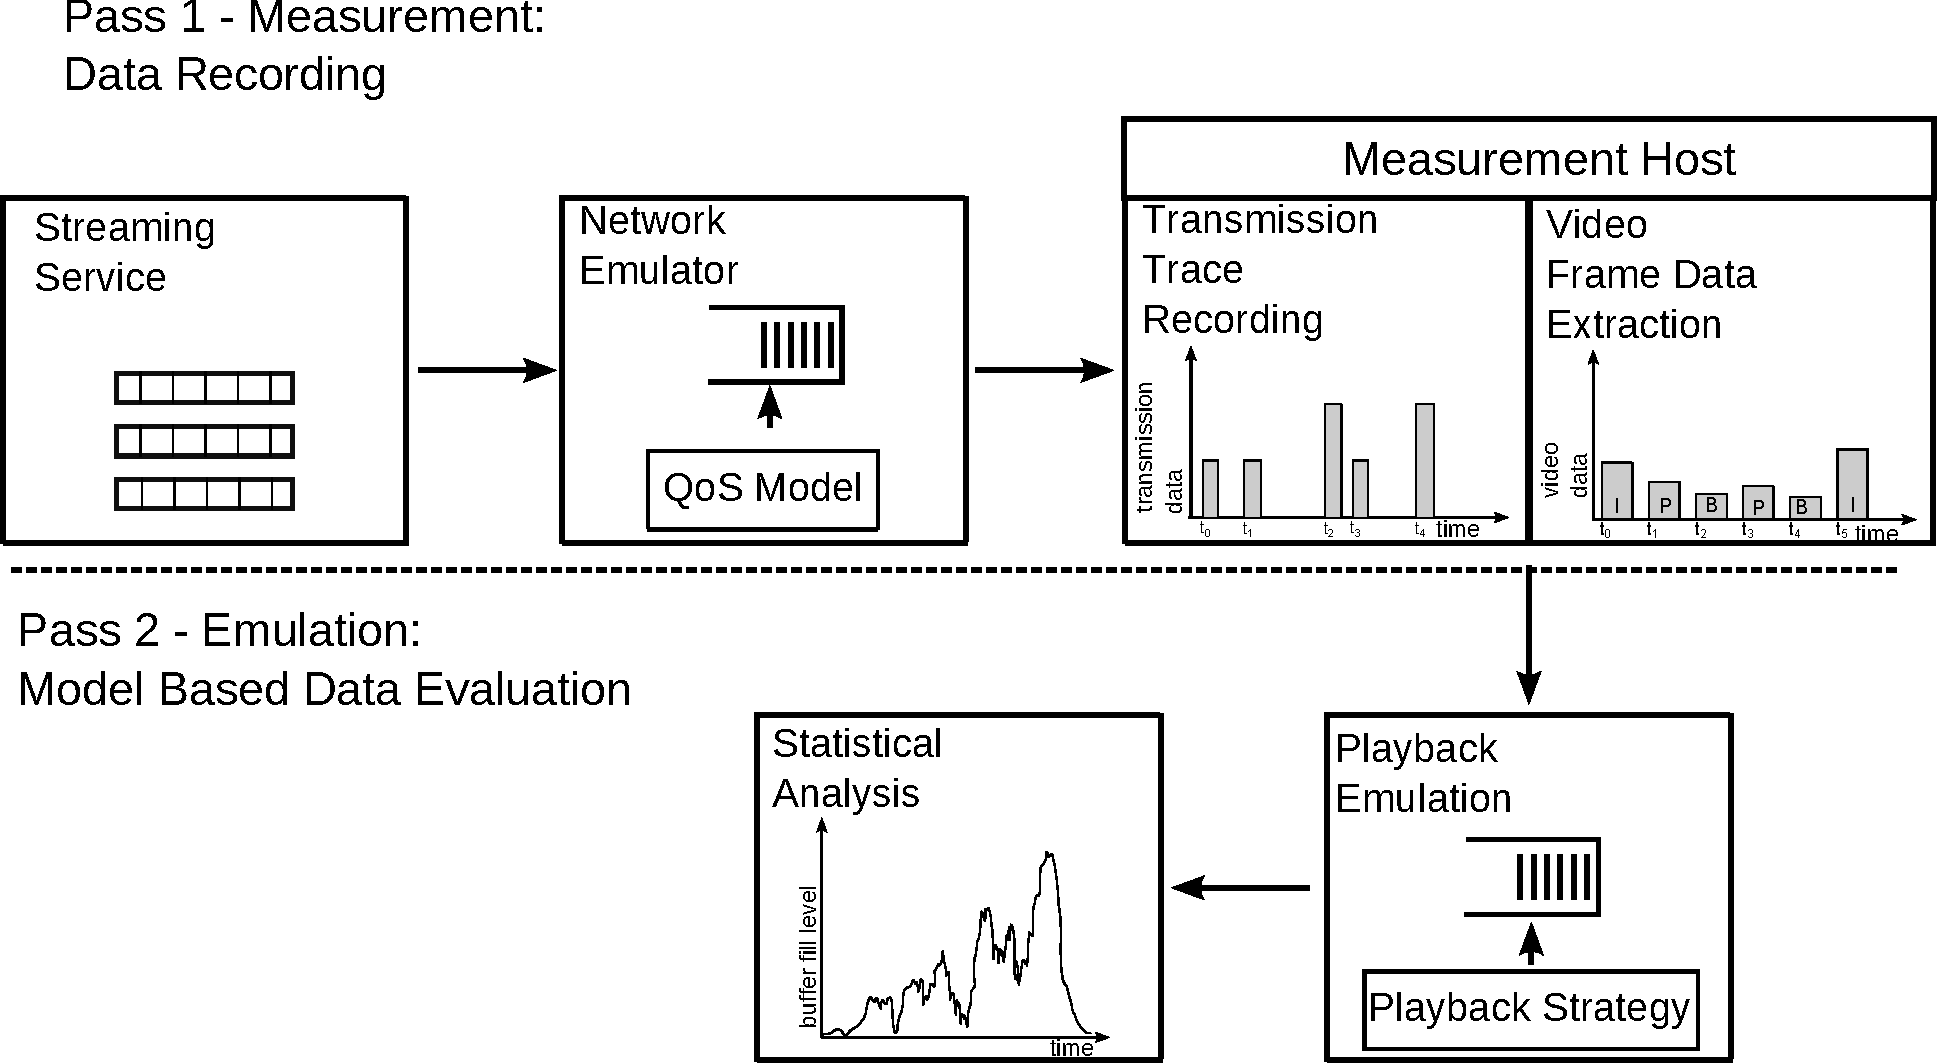
\includegraphics[width=\textwidth]{images/measurement-model.pdf}
    \caption{Measurement framework for progressive streaming playback strategies overview.}
    \label{c3:fig:framework}
\end{figure}

Figure \ref{c3:fig:framework} depicts the framework for a streaming evaluation testbed. In phase one the stream's transmission is conducted and recorded on a per-packet level. Stream data is transmitted to the client from a server which can be any actual streaming service on the Internet or a local server under the testbed's control, eliminating undesired side effects caused by the Internet connection. 

The traffic is directed through a network emulation node capable of altering the network \gls{QoS} parameters, i.e. latency, jitter, and packet loss. The parameters can be set according to stochastic models derived from actual network architectures. Instead of network emulation, any preexisting architecture can also be placed here to achieve more accurate results for the intended target. This is especially helpful for complex infrastructures hard to model or with no good and concise models available yet, for example mobile and mobile core networks with the influence of encapsulating traffic into bearers.

The measurement host downloads and records the video stream as a network trace. For progressive \gls{HTTP} streaming, a single request on the video file is issued and the \gls{TCP} connection maintained until the file has fully arrived.
This process is recorded as basis for the second phase. These traces should consist of the size and timestamp of every incoming packet. More detailed traces can be used to scrutinize other layers of the connection, e.g. the dynamics of TCP receive window size. Additionally the received file is decoded yielding a trace of all video frame sizes and playout timestamps.

In the second pass, these two traces are then used to feed the actual reliable streaming playback model described before. This conducted by a closed-loop emulation process calculating the current buffer fill level based on the collected transmission and video frame traces for every point in time. 

All of the progressive streaming --- i.e. non-adaptive --- strategies can be tested on the same trace set.
In simple \gls{HTTP} streaming, the transmission is not controlled by the streaming application and no rate control is conducted. Therefore, recording the packet trace and simulating playback are completely decoupled, as the latter cannot influence the former.  This enables fast and efficient comparison of non-feedback protocols subject to the same network conditions.

The emulator then generates playback stalling statistics, specifically their number and duration, to compare the effect of the different strategies on the same trace. With these results, parameter settings for playback strategies can also be iteratively tested and improved leading to an empirical calibration of playback strategies instead of relying on best practices.

One of the drawbacks of this model-based emulation approach is of course the reliance on suitable models and playback strategies for the stream protocols under scrutiny. Obtaining these from proprietary streaming clients, can be a difficult reverse-engineering process.


%%
\subsection{Adaptive Streaming Measurement Framework}

Up to this point, the measurement framework is only suitable for progressive streaming omitting any adaptive strategy. This second framework modifies this and additionally allows for the testing of adaptive playback strategies. However, to achieve this, the advantageous two phase setup cannot be employed anymore.

\begin{figure}[htb]
    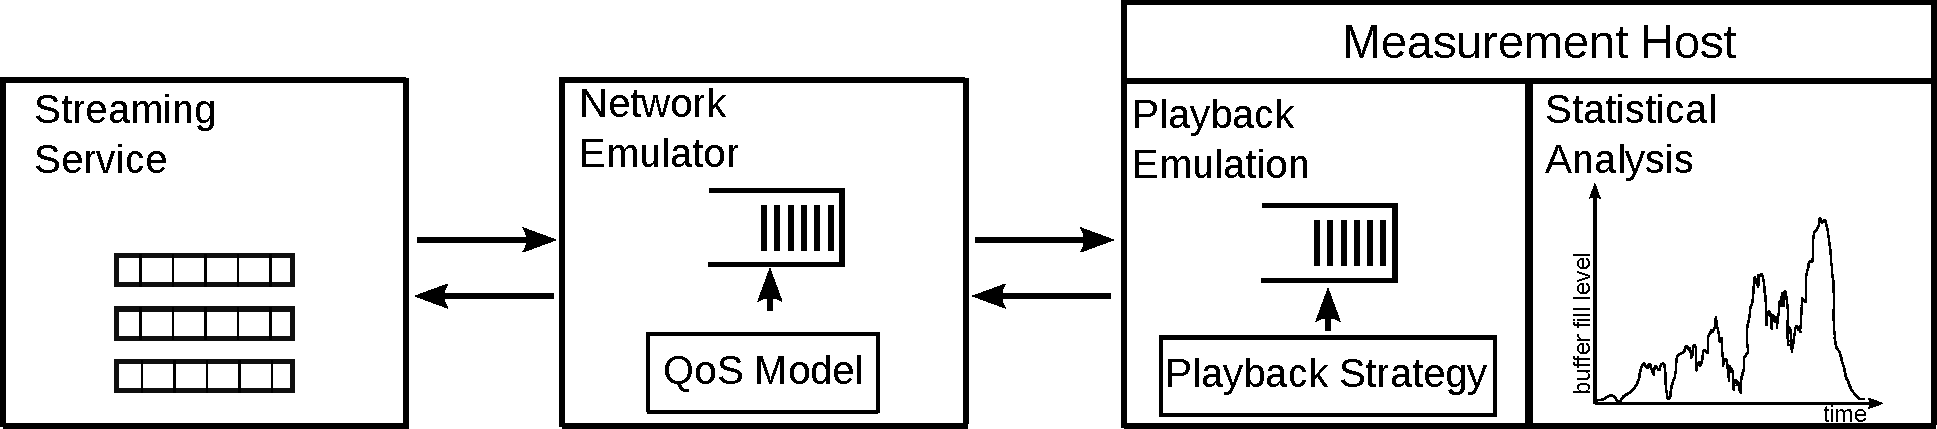
\includegraphics[width=\textwidth]{images/feedback-measurement-model.pdf}
    \caption{Measurement framework for adaptive streaming playback strategies overview.}
    \label{c3:fig:framework-feedback}
\end{figure}

Figure~\ref{c3:fig:framework-feedback} shows the adapted framework. The playback emulation process is now directly fed with the stream transmission without recording it first. The emulation is now an online process and has to be conducted in realtime. This enables the emulator to react on the current streaming state and request an alteration from the server. The adaptation spectrum ranges from the timing of stream segment retrieval to the chosen quality level of future segments. 

While allow for a wider range of playback strategies, this approach is also inherently slower as it does not allow a speed-up beyond realtime, limiting its usability somewhat. Therefore, a transition to a full simulative approach is suggested. This is path is further explored and discussed in Section~\ref{c6:sec:mobilestreamingtestbed}.

\todo{check simulation approach ref or further explain simulation}


%%
\subsection{Technical Implementation}

To conduct measurements, the described two phase progressive streaming measurement framework was implemented in a testbed. This testbed consists of three interconnected physical nodes running Linux. 

The optional streaming server houses an Apache httpd\footnote{\url{https://httpd.apache.org/}} Web server, hosting the files that are to be streamed. Alternatively, Internet streaming service traffic can also be directly routed through the network emulation node.

The network emulation node uses the existing \gls{QoS} capabilities of the Linux kernel, dubbed NetEm \cite{hemminger2005network}, to add latency and packet loss to the transmission as well as to act as a bandwidth bottleneck. The additional delay is set deterministically, the loss follows a uniform distribution without any correlation in the transmission.

To both retrieve the streaming file and record the transmission process at the client, curl\footnote{\url{http://curl.haxx.se/}} is used. If so desired, tcpdump\footnote{\url{http://www.tcpdump.org/}} can also be facilitated to achieve a higher recording precision. The video file is then parsed for its frames and sizes using mplayer\footnote{\url{http://www.mplayerhq.hu/}} with libav\footnote{\url{https://libav.org/}}. The traces are then put into the actual playback emulation, implemented by custom Python-based code and statistically evaluated with Python as well as R.



%%
\subsection{Measurement Series and Evaluations with the Framework}

This implementation has been used to conduct a comparative study of two theoretical and two real world playback strategies. They are tested for their susceptibility to worsening network \gls{QoS}, latency and loss in this case. The evaluated strategies are the described YouTube and Firefox strategies as well as the null strategy and the predictive strategy with perfect knowledge and just the initial stalling period.

The video used in the experiment was streamed from the YouTube web site providing a realistic foundation for the experiments. This also enables a server side pacing mechanism adjusted to the video bitrate for free.
Details on the video used in the experiment are available in Table~\ref{c3:tbl:videoparams}. Two measurement series are performed with this video, both only differ in the network emulator setting. The first series increasingly adds packet loss to the stream, with the second series altering the packet delay. In both scenarios, the link bandwidth was limited to a typical dialup value of \SI{16}{\mega\bit\per\second} in the downlink direction and \SI{1}{\mega\bit\per\second} up.

It can be stated, that all playback strategies will generally work very similar under good network conditions as long as the \gls{TCP} goodput, i.e. the rate the payload is transported by \gls{TCP}, is higher than the video bitrate. With sufficient goodput video streams will start with almost no delay or intermediate buffering. 
If, however, the achievable \gls{TCP} goodput is close to the average video bitrate, the buffer can be quickly drained by short deviations from the average transmission and video bit rates. The \gls{TCP} goodput can be limited by high latency and loss. Many \gls{TCP} congestion control algorithms depend on the round trip time. If the \gls{RTT} is high, the congestion window will increase much slower. High latency triggers \gls{TCP} timeouts and retransmissions, and in turn decrease the congestion window reducing the goodput. Packet loss affects \gls{TCP} goodput even more. A lost packet results in duplicate acknowledgments followed by retransmissions and a decrease of the congestion window. The problem is worsened if the acknowledgments are also lost. The connection could stalls on missing old segments without which the playback cannot proceed. In addition to the reduction of goodput this results in a delay burst and high jitter for the streaming application.


\begin{table}[htbp]
    \centering
    \caption{Test Video Parameters}
    \label{c3:tbl:videoparams}
    \begin{tabu}{X[l]X[r]}
        \toprule
        \textbf{Parameter} & \textbf{Value} \\
        \midrule
        Video Duration  & \SI{92.536}{\second}\\
        Size & \SI{9.61}{\mebi\byte} \\
        Frame rate & \SI{23.976}{\per\second} \\
        Average Video Bitrate & \SI{871}{\kilo\bit\per\second} \\
        Codecs & AVC+AAC \\
        \bottomrule
    \end{tabu}
\end{table}


%% latency
In the latency measurement series, the emulator delays forwarding the packets for a constant amount of time. The latency was increased in \SI{100}{\milli\second} steps, up to a total of \SI{5000}{\milli\second}. The added latency is split up evenly between the uplink and the downlink.

\begin{figure}[htb]
    \centering
    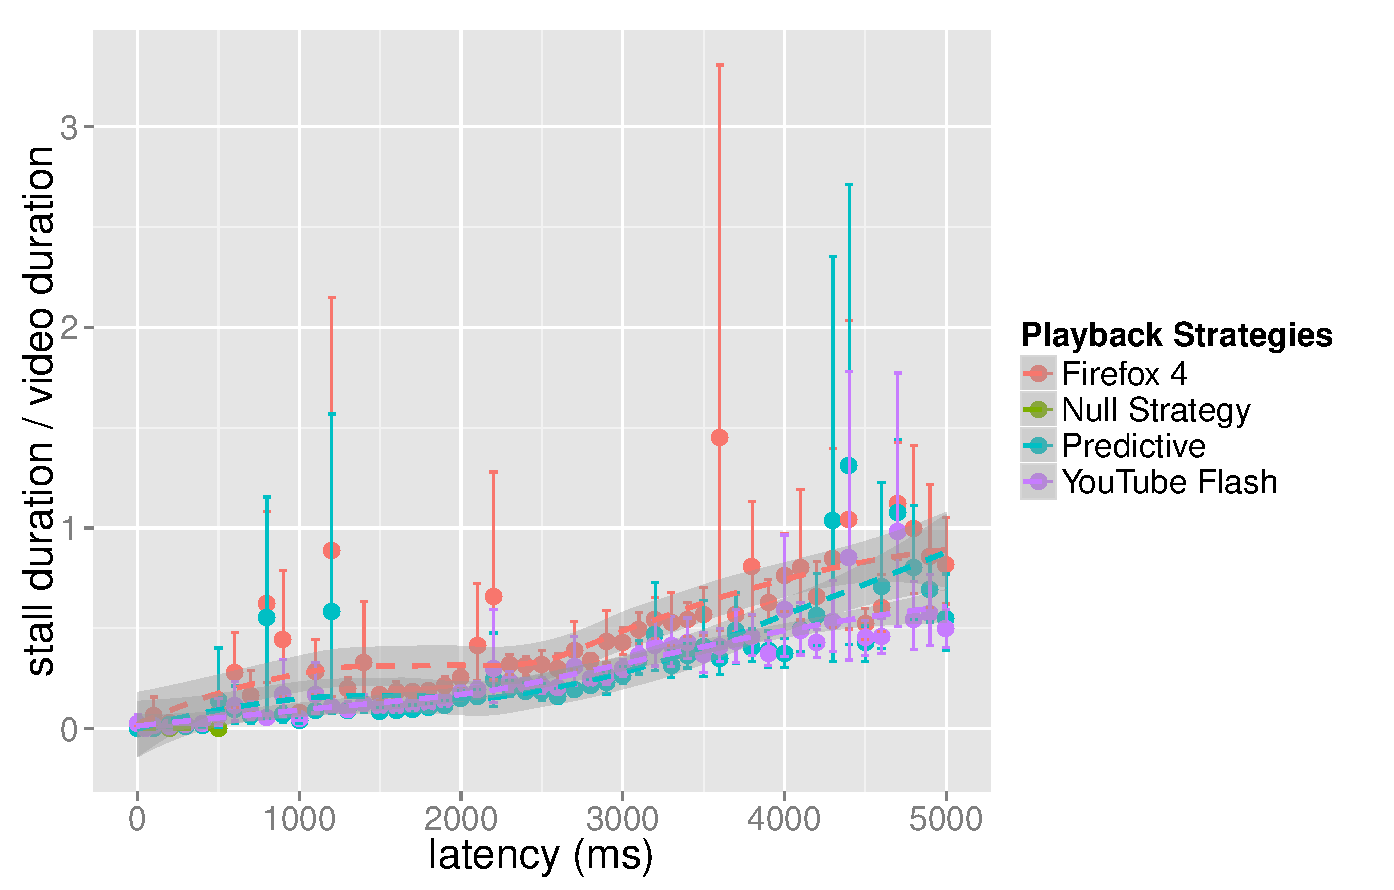
\includegraphics[width=0.9\textwidth]{images/R-playbackemulation-stallduration-latency.pdf}
    \caption{Stalling duration in relation to transmission latency with local polynomial least-squares fit.}
    \label{c3:fig:eval-latency-stallingtime}
\end{figure}


Figure~\ref{c3:fig:eval-latency-stallingtime} depicts the relation between the added latency and the stalling duration of the playback strategies. The stalling time increases as expected with the additional latency, but Firefox's strategy seems to have slight edge during high latency. Overall, the stalling duration quickly reaches a length comparable to the actual video duration and even surpassing that. Someone watching a stream under this condition might find this not acceptable any longer.
% Both the predictive and the null strategy provide the best possible result in terms of pure stalling time. This was already theoretically explored during the strategy's introduction. <-- not true, why?


\begin{figure}[htb]
    \centering
    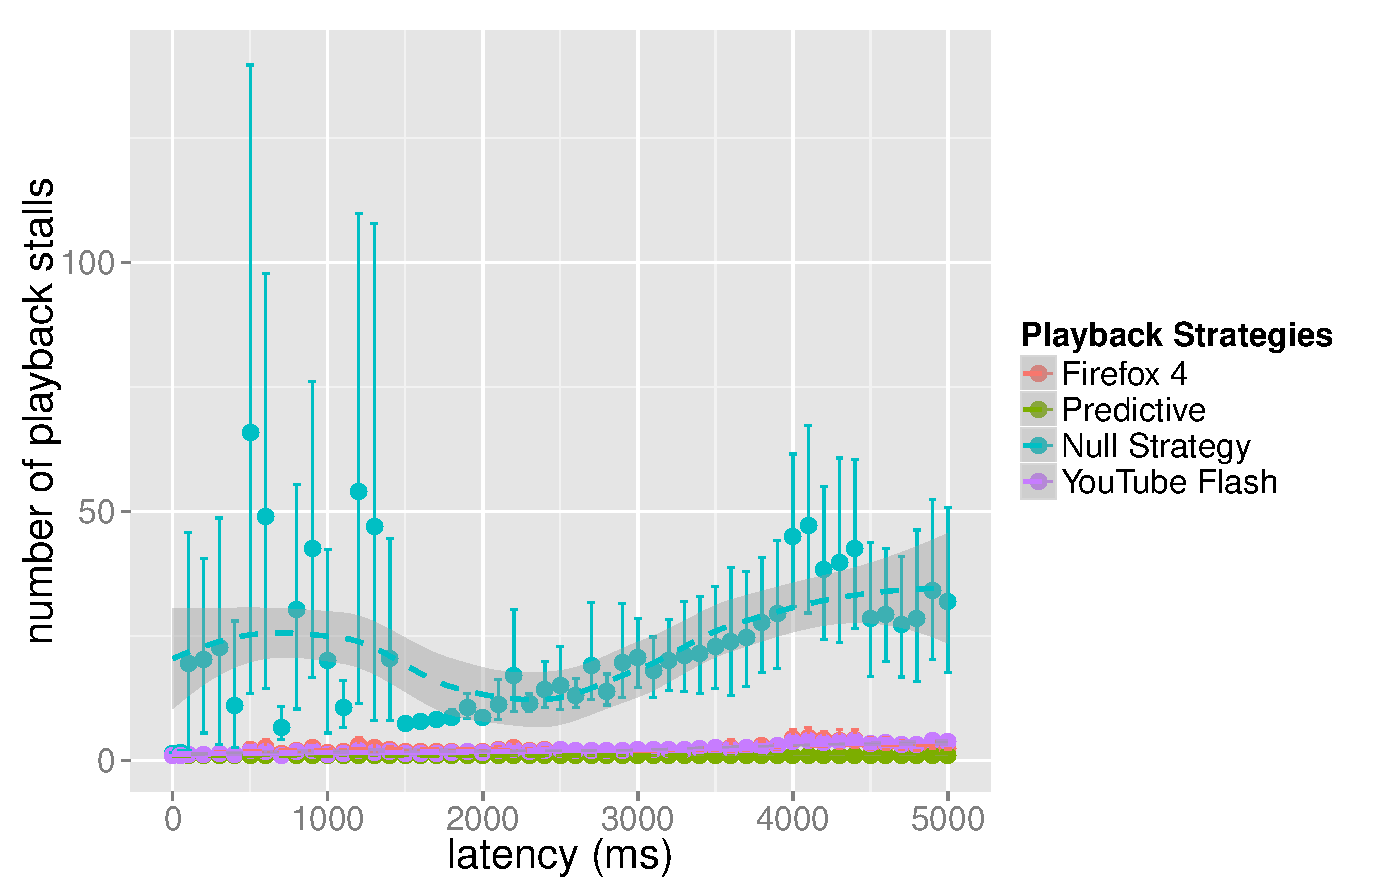
\includegraphics[width=0.9\textwidth]{images/R-playbackemulation-stallnumber-latency.pdf}
    \caption{Number of stalls in relation to transmission latency with local polynomial least-squares fit.}
    \label{c3:fig:eval-latency-numstalls}
\end{figure}

Figure \ref{c3:fig:eval-latency-numstalls} additionally shows number of stalling events occurring during the playback with the null strategy at the high end and the predictive strategy just showing the expected single stall before playback start. %But both YouTube and Firefox are not much worse compared to the predictive strategy, running in just a few buffering events of increasing duration with rising latency. 
%YouTube stalling time is usually lower than with Firefox, at the cost of slightly more buffering events, which could be attributed to its optimistic threshold choice, which still seems to work at the tested latency levels.

Overall, it can be said, that in this specific latency scenario the real world playback strategies seem to honor the fact that more video interruption lead to a worse experience than fewer but longer ones.  Through mobility and handovers, mobile devices experience short bursts of latency of several seconds fairly common. According to the measurement series, the resulting stalling behavior could still very well be bearable for streaming users.

In the loss measurement series, uncorrelated and uniformly distributed loss was added in both the uplink and the downlink direction. The loss was incrementally increased in \SI{2}{\percent} steps up to a total additional loss of \SI{12.5}{\percent}. About \SI{4}{\percent} of the individual experiments did not finish correctly, and the video was not completely transmitted. This was caused by the \gls{TCP} stack, which at some point terminated the connection after to many packets were lost back to back, and curl giving up after several retries. This unpredictability and failure rate also leads to the high variability seen in the results of the loss measurement series. Nonetheless, a certain trend can still be derived from the results.


\begin{figure}[htb]
    \centering
    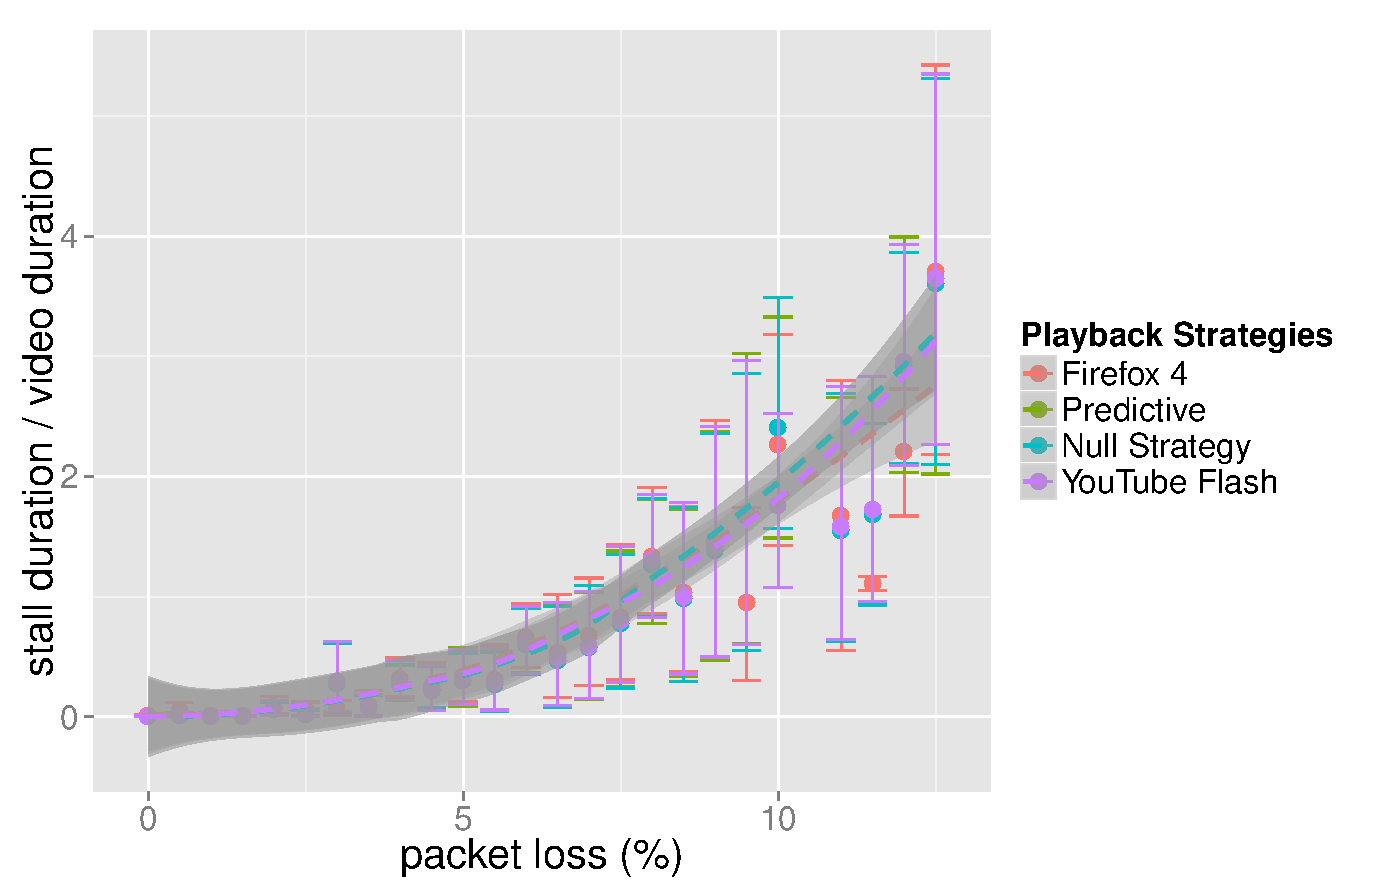
\includegraphics[width=0.9\textwidth]{images/R-playbackemulation-stallduration-loss.pdf}
    \caption{Stalling duration in relation to packet loss with local polynomial least-squares fit.}
    \label{c3:fig:eval-loss-stallingtime}
\end{figure}


Figure~\ref{c3:fig:eval-loss-stallingtime} shows the resulting relative stalling duration in the packet loss measurement series. Loss of up to\SI{4}{\percent} seems to have no discernible impact on the streaming process. Anything beyond this point sees a large increase in the stalling duration. With a relative stalling duration of almost four times the actual video length at \SI{12}{\percent} packet loss any streaming attempt is practically rendered unusable. This behavior could hint to the transport protocol's reliable transport feature, catching any occurring loss. However, the detection and retransmission takes time and leads to a bursty increase in latency offering a possible reason of the increased stalling time.


\begin{figure}[htb]
    \centering
    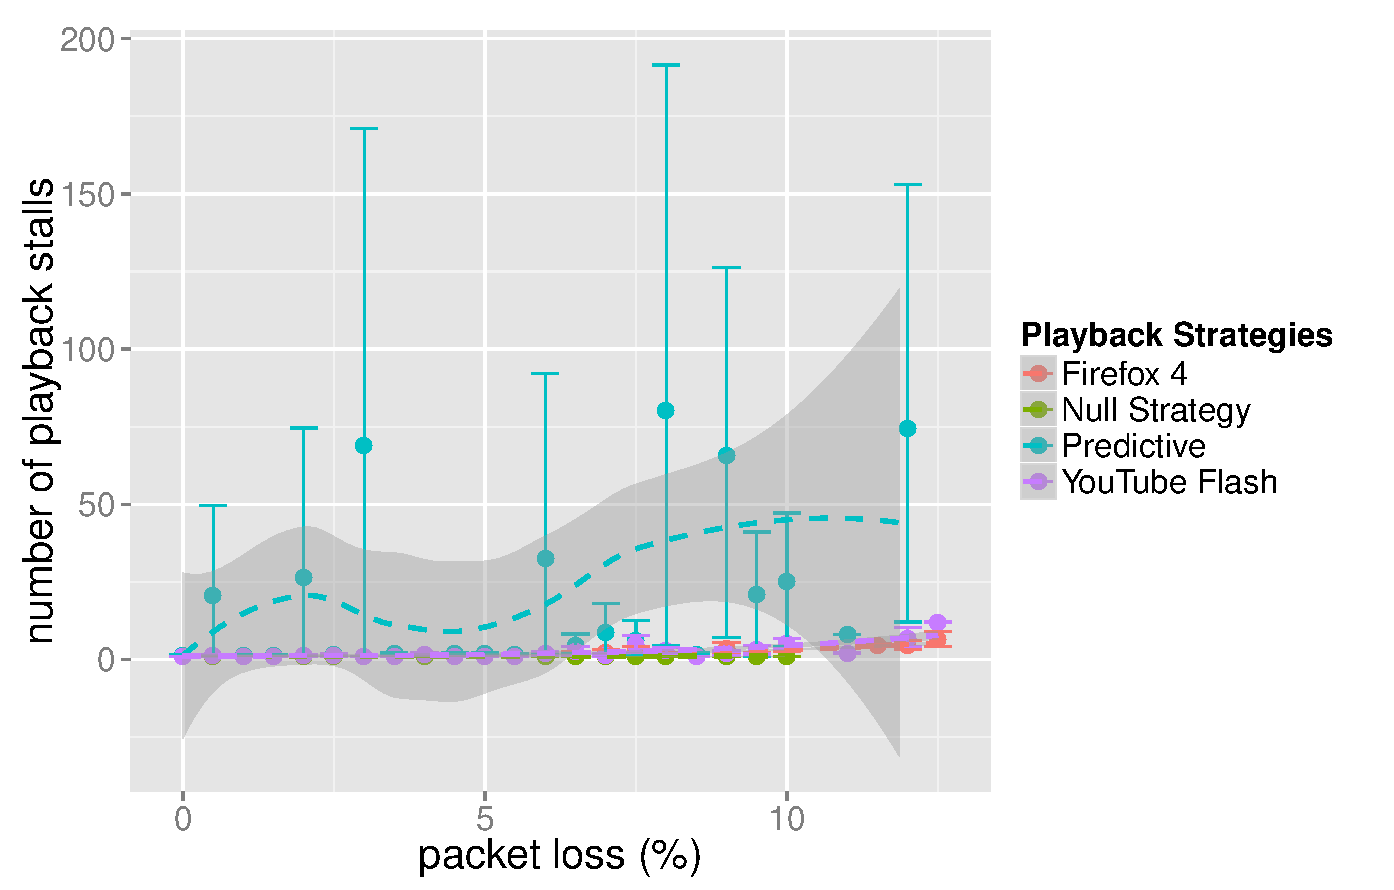
\includegraphics[width=0.9\textwidth]{images/R-playbackemulation-stallnumber-loss.pdf}
    \caption{Number of playback stalls in relation to packet loss with local polynomial least-squares fit.}
    \label{c3:fig:eval-loss-numstalls}
\end{figure}


Figure~\ref{c3:fig:eval-loss-numstalls} shows the extremity of the null strategy in terms of the number of experienced stalls compared to other strategies reaching a number two orders of magnitude larger than any other model. 


As a result, when planning a network for streaming applications, the maximum loss should be kept below the \SI{4}{\percent} mark to achieve reasonable streaming quality. 

\todo{expand loss section a bit more}


%% original python plots
% \begin{figure}[htb]
%     \centering
%     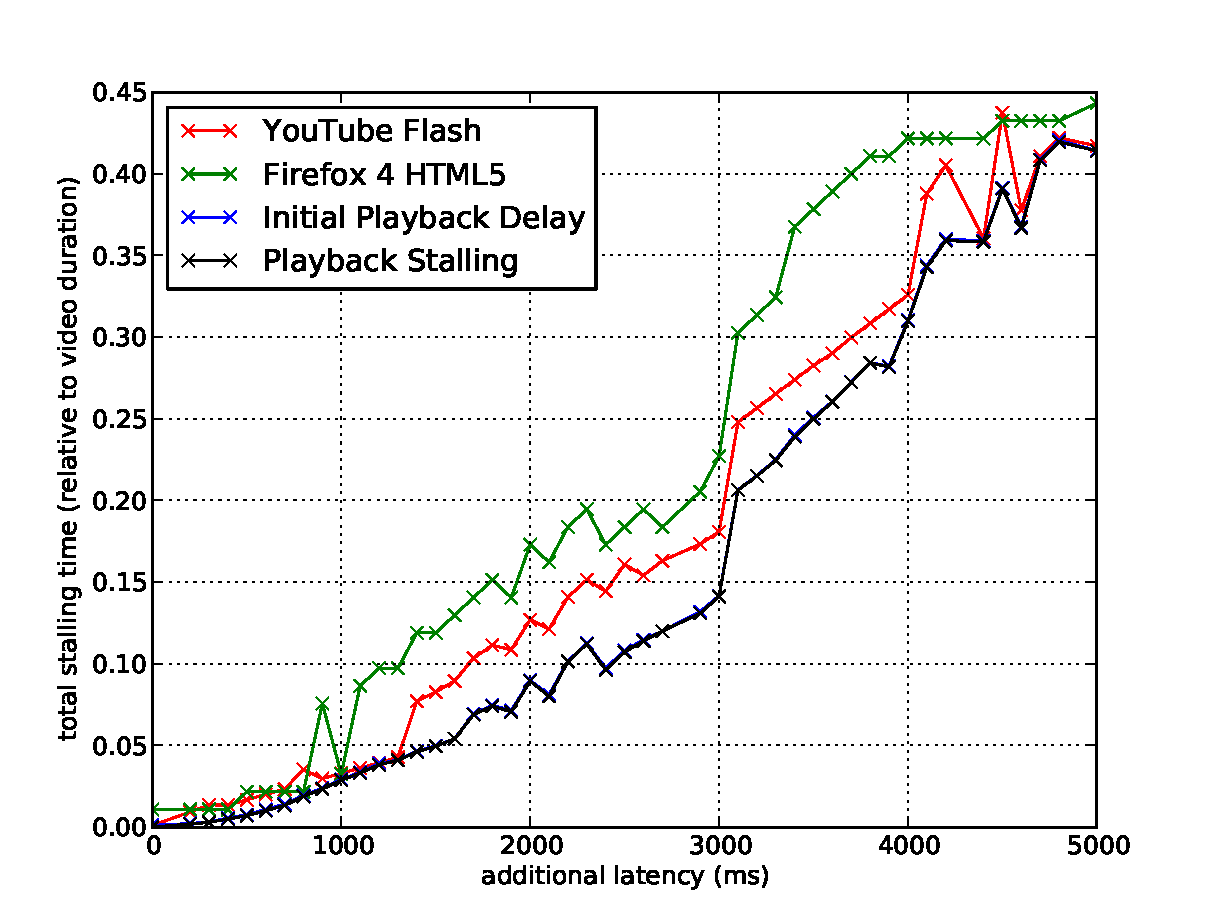
\includegraphics[width=\textwidth]{images/eval-latency-stallingtime.pdf}
%     \caption{Stalling duration in relation to transmission latency.}
%     \label{c3:fig:eval-latency-stallingtime}
% \end{figure}

% \begin{figure}[htb]
%     \centering
%     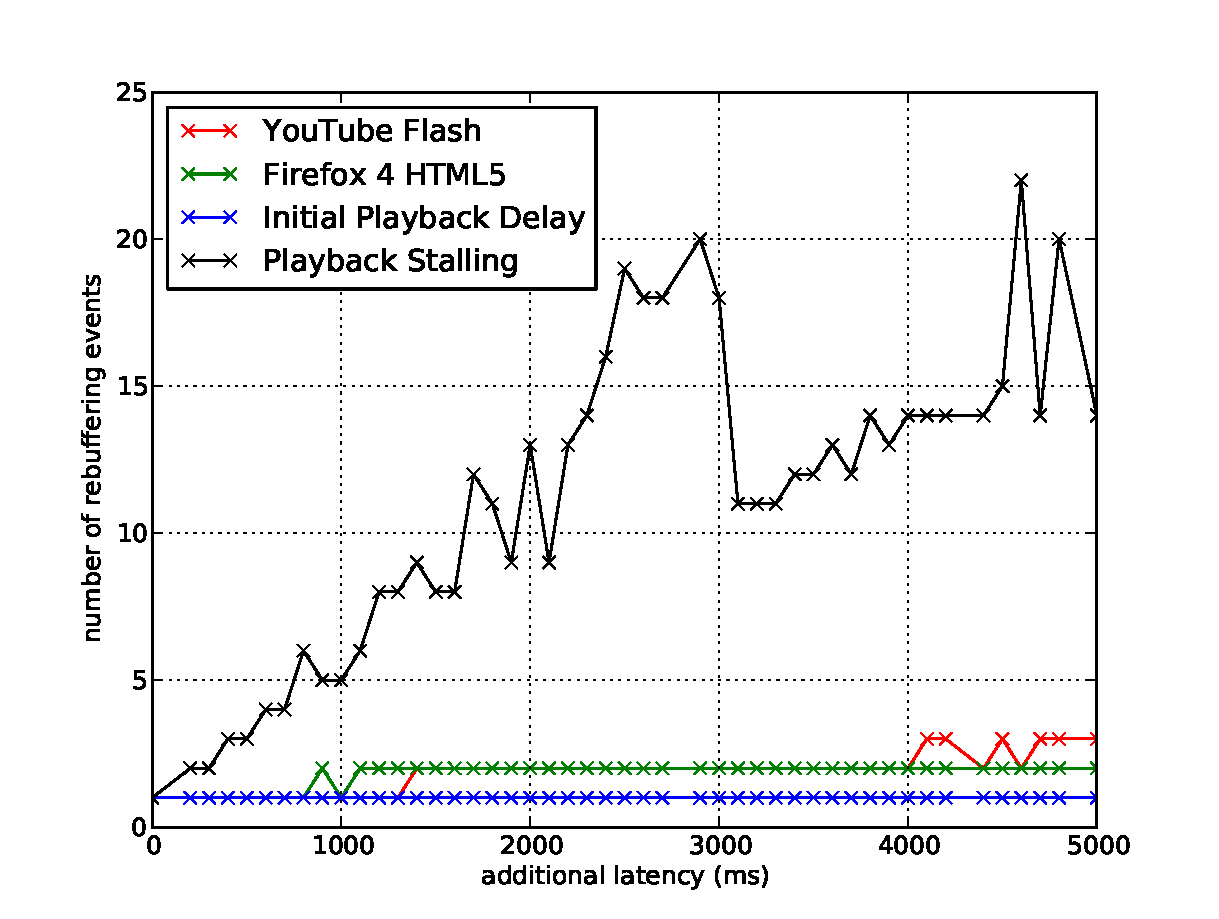
\includegraphics[width=\textwidth]{images/eval-latency-frequency.pdf}
%     \caption{Number of stalls in relation to transmission latency.}
%     \label{c3:fig:eval-latency-numstalls}
% \end{figure}

% \begin{figure}[htb]
%     \centering
%     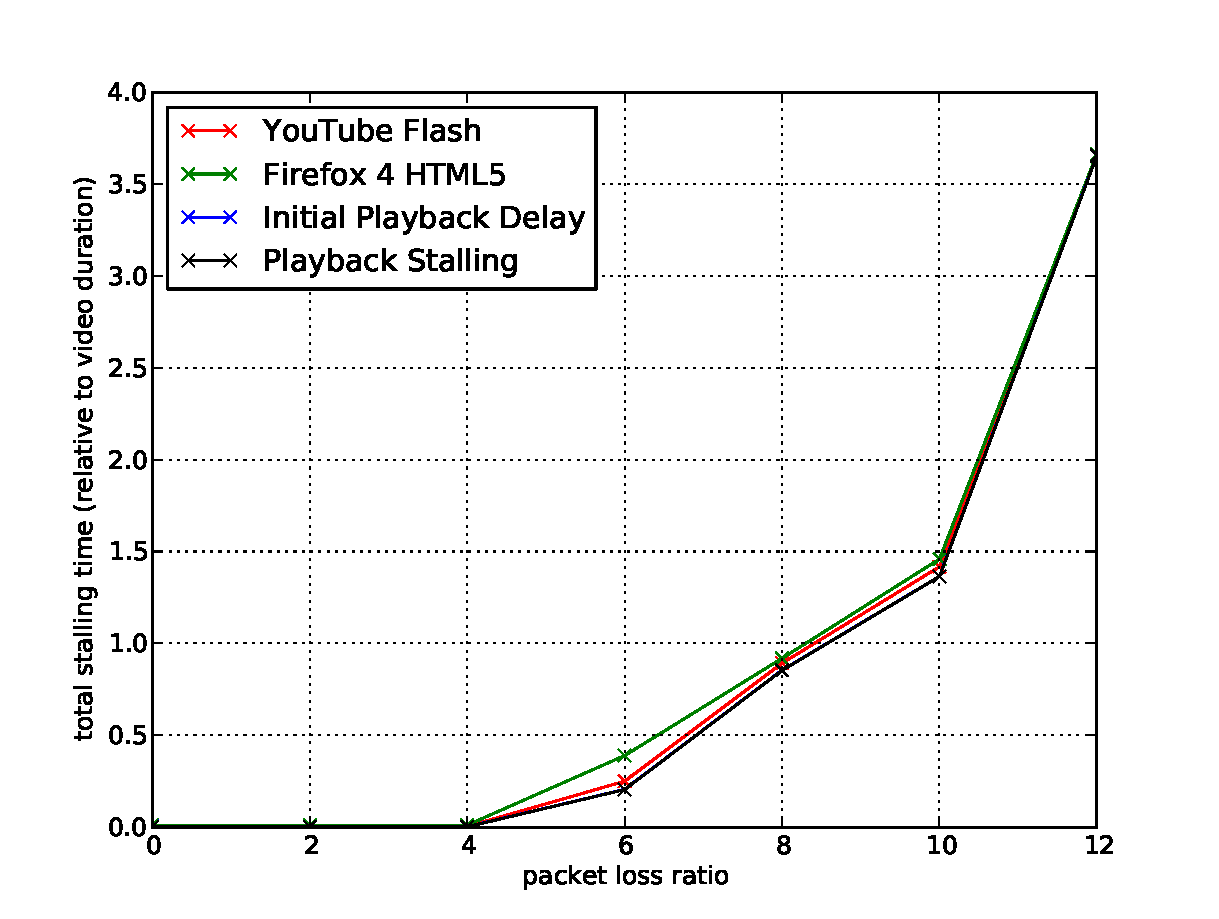
\includegraphics[width=\textwidth]{images/eval-loss4mb-stallingtime.pdf}
%     \caption{Stalling duration in relation to packet loss.}
%     \label{c3:fig:eval-loss-stallingtime}
% \end{figure}

% \begin{figure}[htb]
%     \centering
%     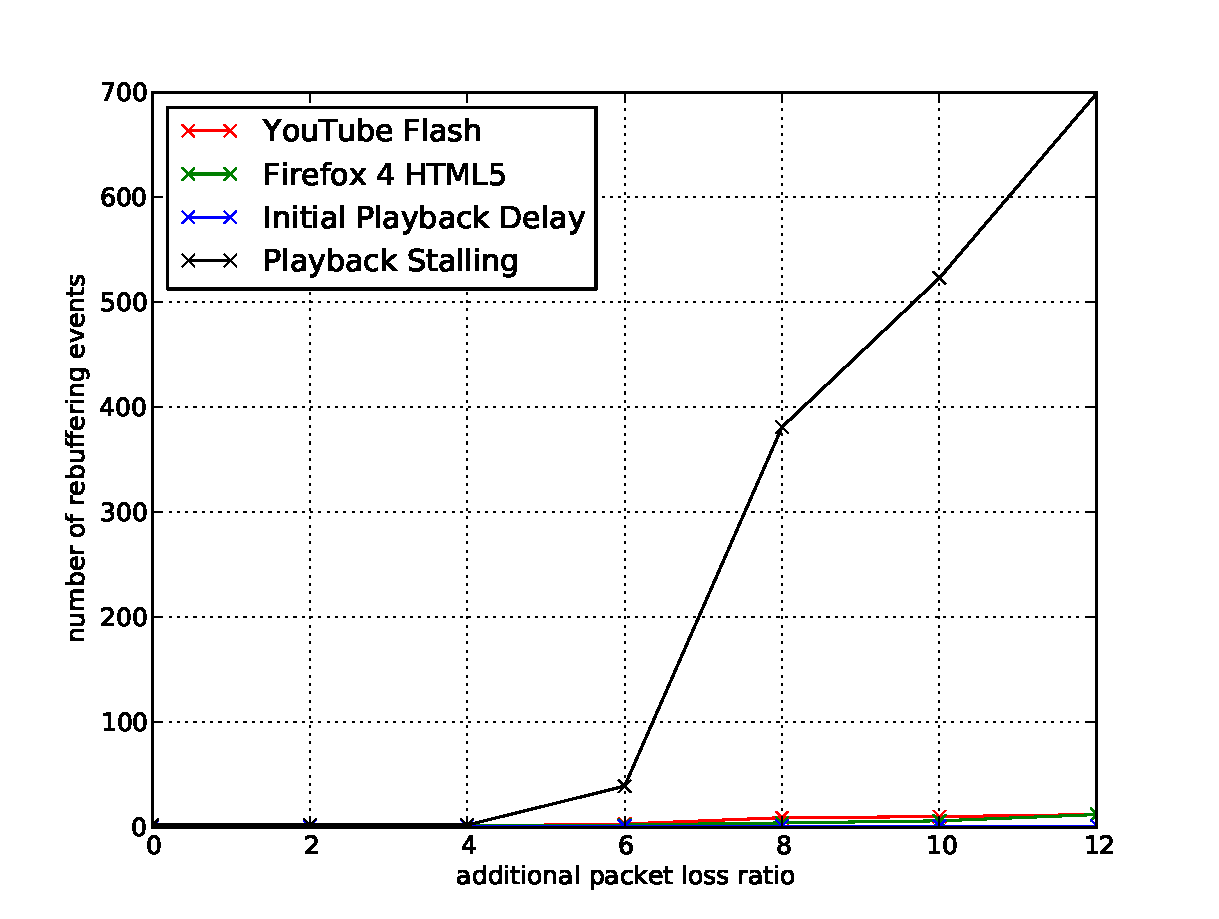
\includegraphics[width=\textwidth]{images/eval-loss4mb-frequency.pdf}
%     \caption{Number of playback stalls in relation to packet loss}
%     \label{c3:fig:eval-loss-numstalls}
% \end{figure}


% \begin{figure}[htbp]
%     \centering
%     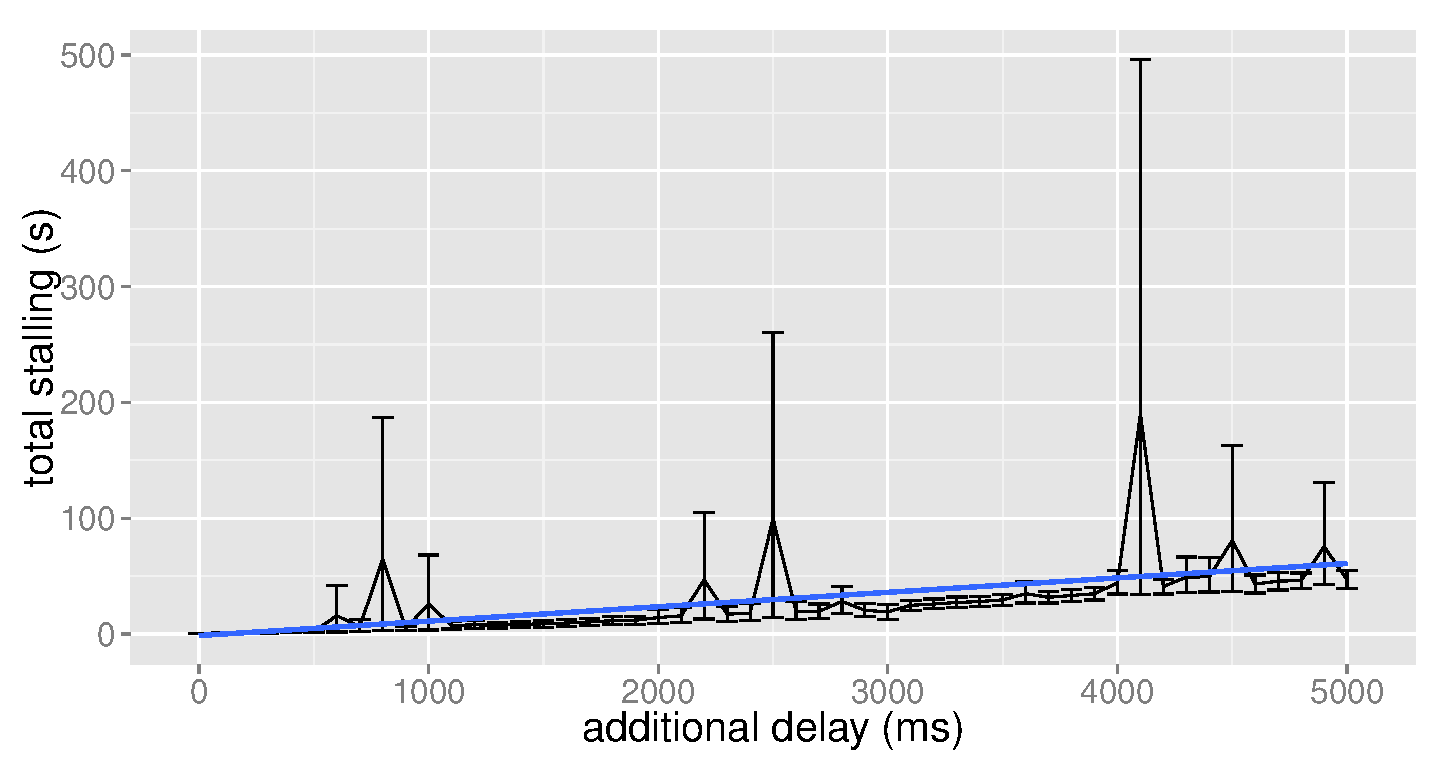
\includegraphics[width=\textwidth]{images/R-delayseries.pdf}
%     \caption{Total buffering time and linear smooth for degraded network parameter scenarios. Latency Graph.}
%     \label{c3:fig:delayseries}
% \end{figure}

% \begin{figure}[htbp]
%     \centering
%     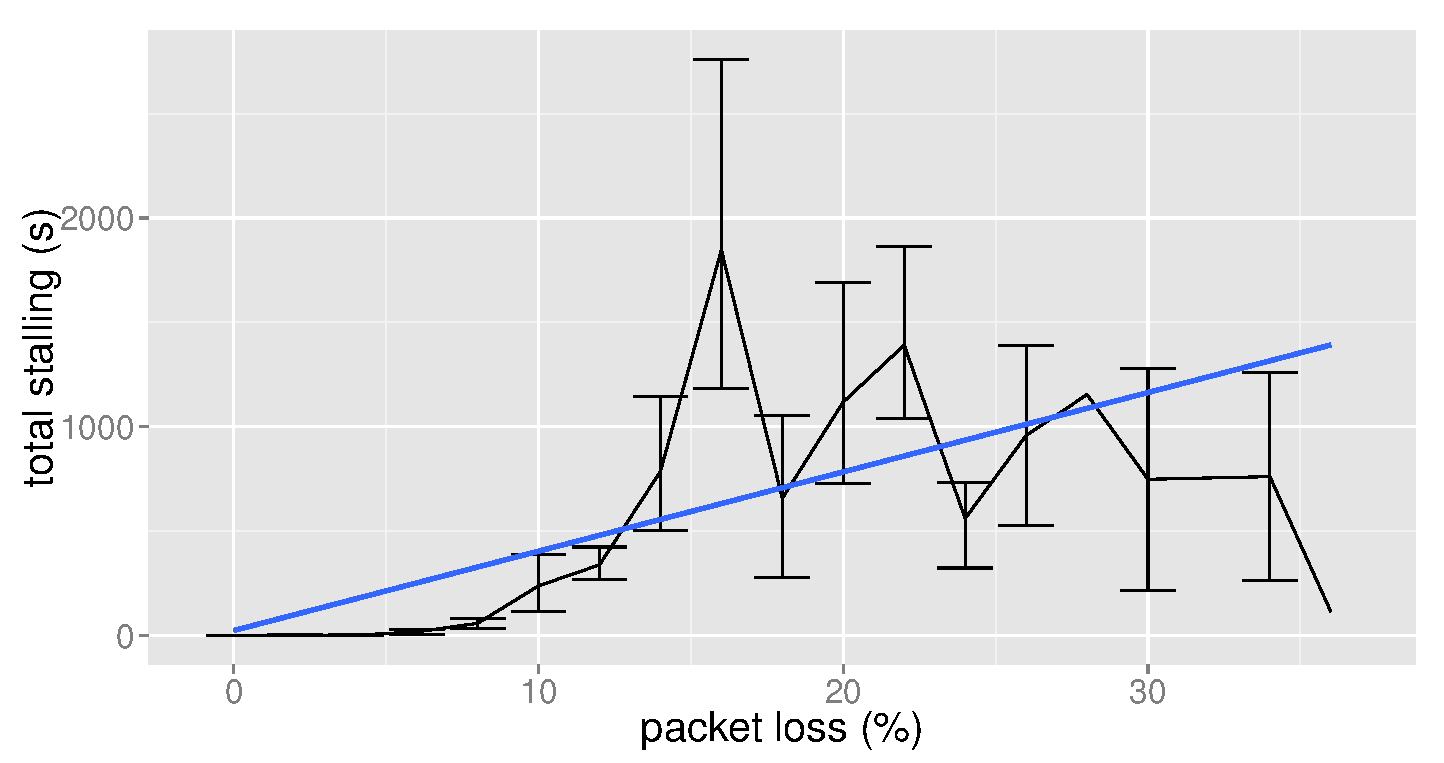
\includegraphics[width=\textwidth]{images/R-lossseries.pdf}
%     \caption{Total buffering time and linear model for degraded network parameter scenarios. Loss Graph.}
%     \label{c3:fig:lossseries}
% \end{figure}



%%%%%%%%%%%%%%%%%%%%%%%%%%%%%%%%%%%%%%%%%%%%%%%%%%%%%%%%%%%%%%%%%%%%%%%%%%%%%%%%
\section{Summary}
\label{c3:sec:conclusion}

Streaming to mobile devices, especially in mobility scenarios, arises several new issues not seen at wireline connected devices. The lower-layer protocols on the radio link can cause additional unexpected behavior. Handover between radio cells can cause long periods of very high delay (up to seconds) and packet reordering which does not play well with TCP, resulting in a decreased throughput. Therefore, we would like to investigate its interplay with server-side bandwidth pacing methods as employed by YouTube.

We also would like to extend our analysis of video streaming to adaptive HTTP streaming mechanisms previously mentioned. We expect them to further complicate the client's buffer management algorithms but they could also serve as a full replacement and evolution to RTP streaming.

In our research we analyzed both the topology as well as the streaming performance of the YouTube platform as a popular example for today's Web-based video delivery. 

With the Seattle platform we actively probed the CDN and discovered several geographical and time-dependent features. Through streaming experiments we have shown that packet loss and delay have considerable influence on the quality of the HTTP video delivery but overall it is reasonably robust to conditions in normal wireline networks. Whether they work as well in wireless networks is a question for future research. Furthermore, we looked at various theoretical and real-world buffering models. We observed that one needs to strike a balance between frequency and length of buffering phases to achieve acceptable playback quality. However, quantizing the quality is also a topic for further research.

%% PV Conclusion
Because of rapid developments in the field of video streaming, full-scale measurement campaigns and analytical modeling might prove too time consuming to test every new protocol. The streaming model framework presented here offers methodologies to quickly evaluate new streaming mechanisms under the influence of network QoS as it decouples the network trace recording and the playback model calculation phase.

We detailed possible influences of the different network layers on video streaming, This inspired the creation of a generic model, incorporating universal notions on data transport, flow control, and buffering, striving to cover most possible streaming methods. Using this model, we explored the theoretical quality limits for streaming such as limits for the maximum stalling duration, and the user trade-offs incurred by making specific choices on how to treat conditions related to streaming processes. In our evaluation of the model on YouTube we observed the influence of network QoS on playback quality and found that high loss is detrimental to HTTP streaming.

The purpose of this model and its evaluations is manifold. It could lead to protocols tailor-made for specific networks or an improved network planning process.
